\documentclass[10pt,a4paper]{article}
\usepackage{blindtext}
\usepackage{subcaption}
\usepackage{graphicx}
\usepackage{tikz}
\usepackage{amssymb}
\usepackage{caption}
\usepackage{amsmath}
\usepackage{circuitikz}
\usepackage{hyperref}
\usepackage{amssymb}
\usepackage[spanish,activeacute,es-tabla]{babel}
\usepackage[utf8]{inputenc}
\usepackage{ifthen}
\usepackage{listings}
\usepackage{dsfont}
\usepackage{subcaption}
\usepackage{amsmath}
\usepackage[strict]{changepage}
\usepackage[top=1cm,bottom=2cm,left=1cm,right=1cm]{geometry}%
\usepackage{color}%
\newcommand{\tocarEspacios}{%
	\addtolength{\leftskip}{3em}%
	\setlength{\parindent}{0em}%
}

% Especificacion de procs

\newcommand{\In}{\textsf{in }}
\newcommand{\Out}{\textsf{out }}
\newcommand{\Inout}{\textsf{inout }}

\newcommand{\encabezadoDeProc}[4]{%
	% Ponemos la palabrita problema en tt
	%  \noindent%
	{\normalfont\bfseries\ttfamily proc}%
	% Ponemos el nombre del problema
	\ %
	{\normalfont\ttfamily #2}%
	\
	% Ponemos los parametros
	(#3)%
	\ifthenelse{\equal{#4}{}}{}{%
		% Por ultimo, va el tipo del resultado
		\ : #4}
}

\newenvironment{proc}[4][res]{%
	
	% El parametro 1 (opcional) es el nombre del resultado
	% El parametro 2 es el nombre del problema
	% El parametro 3 son los parametros
	% El parametro 4 es el tipo del resultado
	% Preambulo del ambiente problema
	% Tenemos que definir los comandos requiere, asegura, modifica y aux
	\newcommand{\requiere}[2][]{%
		{\normalfont\bfseries\ttfamily requiere}%
		\ifthenelse{\equal{##1}{}}{}{\ {\normalfont\ttfamily ##1} :}\ %
		\{\ensuremath{##2}\}%
		{\normalfont\bfseries\,\par}%
	}
	\newcommand{\asegura}[2][]{%
		{\normalfont\bfseries\ttfamily asegura}%
		\ifthenelse{\equal{##1}{}}{}{\ {\normalfont\ttfamily ##1} :}\
		\{\ensuremath{##2}\}%
		{\normalfont\bfseries\,\par}%
	}
	\renewcommand{\aux}[4]{%
		{\normalfont\bfseries\ttfamily aux\ }%
		{\normalfont\ttfamily ##1}%
		\ifthenelse{\equal{##2}{}}{}{\ (##2)}\ : ##3\, = \ensuremath{##4}%
		{\normalfont\bfseries\,;\par}%
	}
	\renewcommand{\pred}[3]{%
		{\normalfont\bfseries\ttfamily pred }%
		{\normalfont\ttfamily ##1}%
		\ifthenelse{\equal{##2}{}}{}{\ (##2) }%
		\{%
		\begin{adjustwidth}{+5em}{}
			\ensuremath{##3}
		\end{adjustwidth}
		\}%
		{\normalfont\bfseries\,\par}%
	}
	
	\newcommand{\res}{#1}
	\vspace{1ex}
	\noindent
	\encabezadoDeProc{#1}{#2}{#3}{#4}
	% Abrimos la llave
	\par%
	\tocarEspacios
}
{
	% Cerramos la llave
	\vspace{1ex}
}

\newcommand{\aux}[4]{%
	{\normalfont\bfseries\ttfamily\noindent aux\ }%
	{\normalfont\ttfamily #1}%
	\ifthenelse{\equal{#2}{}}{}{\ (#2)}\ : #3\, = \ensuremath{#4}%
	{\normalfont\bfseries\,;\par}%
}

\newcommand{\pred}[3]{%
	{\normalfont\bfseries\ttfamily\noindent pred }%
	{\normalfont\ttfamily #1}%
	\ifthenelse{\equal{#2}{}}{}{\ (#2) }%
	\{%
	\begin{adjustwidth}{+2em}{}
		\ensuremath{#3}
	\end{adjustwidth}
	\}%
	{\normalfont\bfseries\,\par}%
}

% Tipos

\newcommand{\nat}{\ensuremath{\mathds{N}}}
\newcommand{\ent}{\ensuremath{\mathds{Z}}}
\newcommand{\float}{\ensuremath{\mathds{R}}}
\newcommand{\bool}{\ensuremath{\mathsf{Bool}}}
\newcommand{\cha}{\ensuremath{\mathsf{Char}}}
\newcommand{\str}{\ensuremath{\mathsf{String}}}

% Logica

\newcommand{\True}{\ensuremath{\mathrm{true}}}
\newcommand{\False}{\ensuremath{\mathrm{false}}}
\newcommand{\Then}{\ensuremath{\rightarrow}}
\newcommand{\Iff}{\ensuremath{\leftrightarrow}}
\newcommand{\implica}{\ensuremath{\longrightarrow}}
\newcommand{\IfThenElse}[3]{\ensuremath{\mathsf{if}\ #1\ \mathsf{then}\ #2\ \mathsf{else}\ #3\ \mathsf{fi}}}
\newcommand{\yLuego}{\land _L}
\newcommand{\oLuego}{\lor _L}
\newcommand{\implicaLuego}{\implica _L}

\newcommand{\cuantificador}[5]{%
	\ensuremath{(#2 #3: #4)\ (%
		\ifthenelse{\equal{#1}{unalinea}}{
			#5
		}{
			$ % exiting math mode
			\begin{adjustwidth}{+2em}{}
				$#5$%
			\end{adjustwidth}%
			$ % entering math mode
		}
		)}
}

\newcommand{\existe}[4][]{%
	\cuantificador{#1}{\exists}{#2}{#3}{#4}
}
\newcommand{\paraTodo}[4][]{%
	\cuantificador{#1}{\forall}{#2}{#3}{#4}
}

%listas

\newcommand{\TLista}[1]{\ensuremath{seq \langle #1\rangle}}
\newcommand{\lvacia}{\ensuremath{[\ ]}}
\newcommand{\lv}{\ensuremath{[\ ]}}
\newcommand{\longitud}[1]{\ensuremath{|#1|}}
\newcommand{\cons}[1]{\ensuremath{\mathsf{addFirst}}(#1)}
\newcommand{\indice}[1]{\ensuremath{\mathsf{indice}}(#1)}
\newcommand{\conc}[1]{\ensuremath{\mathsf{concat}}(#1)}
\newcommand{\cab}[1]{\ensuremath{\mathsf{head}}(#1)}
\newcommand{\cola}[1]{\ensuremath{\mathsf{tail}}(#1)}
\newcommand{\sub}[1]{\ensuremath{\mathsf{subseq}}(#1)}
\newcommand{\en}[1]{\ensuremath{\mathsf{en}}(#1)}
\newcommand{\cuenta}[2]{\mathsf{cuenta}\ensuremath{(#1, #2)}}
\newcommand{\suma}[1]{\mathsf{suma}(#1)}
\newcommand{\twodots}{\ensuremath{\mathrm{..}}}
\newcommand{\masmas}{\ensuremath{++}}
\newcommand{\matriz}[1]{\TLista{\TLista{#1}}}
\newcommand{\seqchar}{\TLista{\cha}}

\renewcommand{\lstlistingname}{Código}
\lstset{% general command to set parameter(s)
	language=Java,
	morekeywords={endif, endwhile, skip},
	basewidth={0.47em,0.40em},
	columns=fixed, fontadjust, resetmargins, xrightmargin=5pt, xleftmargin=15pt,
	flexiblecolumns=false, tabsize=4, breaklines, breakatwhitespace=false, extendedchars=true,
	numbers=left, numberstyle=\tiny, stepnumber=1, numbersep=9pt,
	frame=l, framesep=3pt,
	captionpos=b,
}


\lstset{
    basicstyle=\ttfamily\footnotesize, % Tamaño y tipo de fuente
    keywordstyle=\color{blue},         % Color de las palabras clave
    commentstyle=\color{gray},         % Color de los comentarios
    stringstyle=\color{red},           % Color de las cadenas
    numbers=left,                      % Números de línea a la izquierda
    numberstyle=\tiny\color{gray},     % Estilo de los números de línea
    stepnumber=1,                      % Numerar cada línea
    numbersep=5pt,                     % Separación de los números de línea del código
    tabsize=4,                         % Tamaño de las tabulaciones
    showspaces=false,                  % No mostrar espacios
    showstringspaces=false,            % No mostrar espacios en las cadenas
    breaklines=true,                   % Partir líneas largas automáticamente
    frame=single,                      % Cuadro alrededor del código
    captionpos=b,                      % Poner la leyenda debajo del código
    morekeywords={add, addi, sub, lui, auipc, 
    and, andi, or, ori, xor, xori, li, ret
    sll, slli, srl, srli, sra, srai, 
    slt, slti, sltu, sltiu, 
    beq, bne, blt, bge, bltu, bgeu, 
    jal, jalr, 
    lb, lh, lw, lbu, lhu, 
    sb, sh, sw, 
    fence, fence.i, 
    ecall, ebreak, 
    csrrw, csrrs, csrrc, csrrwi, csrrsi, csrrci, 
    mul, mulh, mulhsu, mulhu, 
    div, divu, rem, remu, 
    flw, fsw, 
    fadd.s, fsub.s, fmul.s, fdiv.s, fsqrt.s, 
    fsgnj.s, fsgnjn.s, fsgnjx.s, 
    fmin.s, fmax.s, 
    fcvt.w.s, fcvt.wu.s, 
    fcvt.s.w, fcvt.s.wu, 
    fmv.x.w, fmv.w.x, 
    feq.s, flt.s, fle.s, 
    fclass.s}      
}

\title{Sistemas Digitales}
\author{Tomás Agustín Hernández}
\date{}

\begin{document}
\maketitle


\begin{figure}[b]
    \centering
    \begin{tikzpicture}[remember picture,overlay]
        \node[anchor=south east, inner sep=0pt, xshift=-1cm, yshift=2cm] at (current page.south east) {
            \begin{minipage}[b]{0.5\textwidth}
                
\includegraphics[width=\linewidth]{logo_uba.jpg}
                \label{fig:bottom}
            \end{minipage}
        };
    \end{tikzpicture}
\end{figure}

\newpage

\section{Introducción a los sistemas de representación}
\subsection*{Magnitud}
Llamamos magnitud al tamaño de algo, dicho en una medida específica. 
Es representada a través de un sistema que cumple 3 conceptos fundamentales: 
\begin{itemize}
    \item Finito: Debe haber una cantidad finita de elementos.
    \item Composicional: El conjunto de elementos atómicos deben ser fáciles de implementar y componer.
    \item Posicional: La posición de cada dígito determina en qué proporción modifica su valor a la magnitud total del número.
  \end{itemize}
Algunos de los sistemas de representación más utilizados son: binario, octal, decimal y hexadecimal.

\subsection*{Bases}
Una base nos indica la cantidad de símbolos que podemos utilizar para poder representar determinada magnitud.
\begin{table}[h!]
    \centering
    \begin{tabular}{|c | c|}
    \hline
    \textbf{Base} & \textbf{Símbolos disponibles}  \\[0.1cm]
    \hline\hline
    2 (binario) & 0, 1 \\
    8 (octal) & 0, 1, 2, 3, 4, 5, 6, 7 \\
    10 (decimal) & 0, 1, 2, 3, 4, 5, 6, 7, 8, 9 \\
    16 (hexadecimal) & 0, 1, 2, 3, 4, 5, 6, 7, 8, 9, A, B, C, D, E, F \\
    \hline
    \end{tabular}
    \caption{Bases más utilizadas}
    \label{tab:bases}
\end{table}

La tabla anterior representa los símbolos disponibles para las bases 2, 8, 10 y 16.\\


Consideremos por un momento que estamos en binario; ¿sería correcto que 1 + 1 = 2? ¡No! Porque 2 no es un símbolo válido en base 2.\\

Para indicar la base en la que está escrito un número, se coloca la base entre paréntesis en la esquina inferior derecha.\\

\(1024_{(10)}\): 1024 representado en base 10 (decimal) \\

\textbf{Importante}: 1 dígito hexadecimal son 4 bits en binario. \\
\textbf{Importante 2}: Cuando vemos 0x123456 en RISC-V solo se considera 123456 si necesitamos hacer cualquier operación, el 0x indica solamente que está en hexadecimal.

    
\subsection*{Digítos/Bits}
Sea \( n \in \mathbb{Z} \), cuando decimos que tenemos n bits es lo mismo que decir que tenemos n dígitos.
\\
\begin{itemize}
\item 0001: Representa el número 1 en binario, en 4 bits/dígitos.
\item 0010: Representa el número 2 en binario, en 4 bits/dígitos.
\end{itemize}

\subsection*{Teorema de división}
Es una manera de poder realizar un cambio de base de un número decimal a otra base. La representación en la otra base es el resto visto desde abajo hacia arriba.

\[a = k \ast d + r \ con \ 0 \le r < \longitud{d}\] donde:
\begin{itemize}
    \item k = cociente
    \item d = divisor.
    \item r = resto de la división de a por d.
  \end{itemize}

Pasaje del número \(128_{(10)}\) a \(128_{(2)}\) en 8 bits

\[128 = 64 \ast 2 + 0\]
\[64 = 32 \ast 2 + 0\]
\[32 = 16 \ast 2 + 0\]
\[16 = 8 \ast 2 + 0\]
\[8 = 4 \ast 2 + 0\]
\[4 = 2 \ast 2 + 0\]
\[2 = 1 \ast 2 + 0\]
\[1 = 0 \ast 2 + 1\]

Luego, \(128_{(2)}\) = 1000 0000

\subsection*{Bit más significativo / menos significativo}
El bit más significativo en un número es el que se encuentra a la izquierda, mientras que el menos significativo es el que se encuentra a la derecha.
\[\textcolor{blue}{\textbf{1}}000 000\textcolor{blue}{\textbf{0}}_{(2)}\]


\subsection*{Tipos numéricos}
Representemos números naturales y enteros a partir de la representación en base 2 (binario) \\

\textbf{Sin signo}: Representa únicamente números positivos. No se pueden utilizar los símbolos de resta (\textbf{-}) ni tampoco coma (\textbf{,})
\[1_{(10)} = 01_{(2)}\]
\[128_{(10)} = 1000 0000_{(2)}\]

\textbf{Signo + Magnitud}: Nos permite representar números negativos en binario. \\ El bit más significativo indica el signo
\begin{itemize}
    \item 0: número positivo
    \item 1: número negativo.
\end{itemize}

\[18_{(10)} = \textcolor{blue}{\textbf{0}}0010010_{(2)}\]
\[-18_{(10)} = \textcolor{blue}{\textbf{1}}0010010_{(2)}\]

Representar números en S+M suele traer problemas porque el 0 puede representarse de dos maneras
\[+0_{(10)} = \textcolor{blue}{\textbf{0}}0000000_{(2)}\]
\[-0_{(10)} = \textcolor{blue}{\textbf{1}}0000000_{(2)}\]

Para solucionar este problema, las CPU utilizan la notación Complemento a 2 \((C_{2})\) \\

\textbf{Exceso m}: Sea \( m \in \mathbb{Z} \), decimos que un número n está con exceso \(m\) unidades cuando \(m>0\) 
\[n_{0}=n+m\]
\[n=1 \land m=10 \implica n_{0}=-9 \]
Nota: \(n_{0}\) indica el valor original de \(n\)  antes de ser excedido \(m\) unidades.  \\

\textbf{Complemento a 2}: Los positivos se representan igual. \\ 
El bit más significativo indica el signo, facilitando saber si el número es positivo o negativo.
Cosas a tener en cuenta
\begin{itemize}
    \item \textbf{Rango}: \( -2^{n-1} \ hasta \ 2^{n-1}-1 \)
    \item \textbf{Cantidad} de representaciones del cero: Una sola
    \item \textbf{Negación}: Invierto el número en representación binaria positiva y le sumo uno.
    \begin{itemize}
        \item \(-2_{(2)} = inv(010) + 1\)
        \item \(-2_{(2)} = 101 + 1\)
        \item \(-2_{(2)} = 110\)
    \end{itemize}
    \item \textbf{Extender número a más bits}: Se rellena a la izquierda con el valor del bit del signo.
    \item \textbf{Regla de Desbordamiento}: Si se suman dos números con el mismo signo, solo se produce desbordamiento cuando el resultado tiene signo opuesto.
\end{itemize}

\subsection*{Overflow / Desbordamiento}
Hablamos de overflow/desbordamiento cuando 
\begin{itemize}
    \item\label{item:overflow1} El número a representar en una base dada, excede la cantidad de bits que tenemos disponibles.
    \item\label{item:overflow2} Si estamos en notación \(C_{2}\) al sumar dos números cambia el signo.
\end{itemize} 


\subsection*{Acarreo / Carry}
Ocurre cuando realizamos una suma de números binarios y el resultado tiene más bits que los números originales que estamos sumando

\subsection*{Borrow}
Borrow \(\equiv\) Préstamo. \\
Se produce cuando el sustraendo (denominador) es mayor que el minuendo (numerador) por lo tanto se debe pedir.

\begin{lstlisting}
      0111
    - 1000
      ====
      1011

      El primer cero le pide al uno de su derecha.
\end{lstlisting}

\subsection*{Suma entre números binarios}
Se hace exactamente igual que una suma común y corriente. \\
Es importante prestar atención a la cantidad de dígitos que nos piden para representarlo, y en caso de estar en \(C_{2}\) que el signo no cambie.\\ 
\\
Hagamos sumas en \(C_{2}\) (sin límite de bits)

\begin{align*}
    &\begin{array}{@{} r@{}}
      0010 = 2 \\
    + 1001 = -7\\
    \hline
    \ 1011 = -5
    \end{array}
    &&
    \begin{array}{@{} r @{}}
       0101 = 5 \\
    + 1110 = -2 \\
    \hline
    \textcolor{blue}{\textbf{1}}0011 = 3
    \end{array}
    &&
    \begin{array}{@{} r @{}}
       1011 = -5 \\
    + 1110 = -2 \\
    \hline
    \textcolor{blue}{\textbf{1}}1001 = -7
    \end{array}
    &&
    \begin{array}{@{} r @{}}
       0111 = 7 \\
    + 0111 = 7\\
    \hline
    \textcolor{red}{\textbf{1}}110 = \text{Overflow}
    \end{array}
    &&
    \begin{array}{@{} r @{}}
       1010 = -6 \\
    + 1100 = -4 \\
    \hline
    \textcolor{blue}{\textbf{1}}\textcolor{red}{\textbf{0}}110 = \text{Overflow}
    \end{array}
    \end{align*}

Nota: El color azul indica el carry; El rojo indica qué es lo que produce overflow (cambio de signo).
\\
\\
Hagamos sumas en \(C_{2}\) (límite de bits: 4)

\begin{align*}
    &\begin{array}{@{} r@{}}
      0010 = 2 \\
    + 1001 = -7\\
    \hline
    \ 1011 = -5
    \end{array}
    &&
    \begin{array}{@{} r @{}}
       0101 = 5 \\
    + 1110 = -2 \\
    \hline
    \textcolor{blue}{\textbf{1}}0011 = Overflow
    \end{array}
    &&
    \begin{array}{@{} r @{}}
       1011 = -5 \\
    + 1110 = -2 \\
    \hline
    \textcolor{blue}{\textbf{1}}1001 = Overflow
    \end{array}
    &&
    \begin{array}{@{} r @{}}
       0111 = 7 \\
    + 0111 = 7\\
    \hline
    \textcolor{red}{\textbf{1}}110 = \text{Overflow}
    \end{array}
    &&
    \begin{array}{@{} r @{}}
       1010 = -6 \\
    + 1100 = -4 \\
    \hline
    \textcolor{blue}{\textbf{1}}\textcolor{red}{\textbf{0}}110 = \text{Overflow}
    \end{array}
    \end{align*}

Nota: Al tener un límite de 4 bits, en las sumas que tenemos carry terminamos teniendo overflow.
\subsection*{Resta entre numeros binarios}
La resta entre números binarios debe realizarse en \(C_{2}\)

La idea es que A - B \(\equiv\) A + (INV(B) + 1) 
\subsection*{¿Cuando hay overflow, carry o borrow?}
\begin{itemize}
    \item POS + POS = NEG
    \item NEG + NEG = POS
    \item POS - NEG = NEG
    \item NEG - POS = POS 
\end{itemize}
\begin{lstlisting}
      0101
    + 0110
      ====
      1011  - OV: si - C: no

      1000
    + 1100
      ====
      10100 - OV: si - Carry si

      1010
    - 0100
      ====
      1000 - OV: si - Borrow no

      0100
    - 1000
      ====
      1000 - OV: si - Borrow si
\end{lstlisting}
\subsection*{Rango de valores representables en n bits}
Sean \( n, m \in \mathbb{Z} \) decimos que el rango de representación en base \(n\) y \(m\) bits acepta el rango de valores de: 
\(
\left[ -n^m, n^m - 1 \right]
\)

¿Es posible representar el 1024 en binario y 4 bits? No.
\begin{itemize}
    \item \(2^4\) = 16 \(\implies [-16, 15]\)
    \item Pero, 1024 \(\notin [-16, 15]\)
    \item Por lo tanto, 1024 no es representable en 4 bits.
\end{itemize} 

\subsection*{Pasar número binario a decimal}
1. Si tenemos el mismo número todo el tiempo podemos usar la serie geométrica \\

¿Qué número decimal representa el número \(1111111111_{(2)}\)?
\[
\begin{array}{l}
\sum_{i=0}^{j-1} 1 \cdot n^i = \begin{array}{@{} r @{}}
    q^{n+1} - 1 \\
    \hline
    q-1
 \end{array}
\end{array}
Luego, 
\]
\[
\begin{array}{l}
\sum_{i=0}^{9} 1 \cdot 2^i = \begin{array}{@{} r @{}}
    2^{10} - 1 = 1023 \\
 \end{array}
\end{array}
\]

2. Si no tenemos el mismo número todo el tiempo podemos multiplicar cada dígito por la base donde el exponente es la posición del bit. \\

\(10_{(2)} = 1 \ast 2^{1} + 0 \ast 2^{0} = 2_{(10)} \)

\subsection*{Extender un número de n bits a m bits}
Sea \( n, m \in \mathbb{Z} \) donde \(n\) es la cantidad de bits inicial y \(m\) es la cantidad a la que se quiere extender.
\[n = 3 \land m = 8\]

\begin{itemize}
    \item Signo + Magnitud y exceso m: Se extiende con 0's luego del signo.
    \begin{itemize}
        \item En 3 bits, -2 = 110
        \item En 8 bits, -2 = \textcolor{blue}{\textbf{1}}\textcolor{cyan}{\textbf{00000}}10
    \end{itemize}
    \item Complemento 2 (\(C_{2}\)): Se extiende con el bit más significativo.
    \begin{itemize}
        \item En 3 bits, -2 = 110
        \item En 8 bits, -2 = \textcolor{blue}{\textbf{1}}\textcolor{cyan}{\textbf{11111}}10
    \end{itemize}
\end{itemize} 

\subsection*{Cambios de base} 
Sea \( n, m \in \mathbb{Z} \) dos bases distintas, para pasar de base \(n\) a base \(m\) se debe realizar el siguiente proceso

\begin{itemize}
    \item Pasar el número a base decimal.
    \item Aplicar el teorema de división utilizando la base deseada.
\end{itemize}

Encontremos en base 5, el número que corresponde a \(17_{(8)}\):
\begin{itemize}
    \item  \( 17_{(8)} = 1 \ast 8^{1} + 7 \ast 8^{0} = 15_{(10)} \)
    \item Usando ahora el teorema de división
    \begin{itemize}
    \item  \( 15 = 3 \ast 5 + 0 \)
    \item  \( 3 = 0 \ast 5 + 3 \)
    \item Luego, \( 30_{(5)} \)
    \end{itemize} 
    \item Por lo tanto, \( 17_{(8)} = 30_{(5)} \)
\end{itemize} 

\section{Desplazamientos}
Utilizamos los desplazamientos para poder mover los bits. Cada casillero representa los bits.
\begin{itemize}
    \item Desplazamiento hacia la izquierda: Se desplazan los bits del dato tantas posiciones como se indiquen a la izquierda. \\
     \(variable << cantidad\)\\ \begin{minipage}[b]{0.32\textwidth}
        \includegraphics[width=\linewidth]{assets/desplazamiento_izquierda.png}
        \label{fig:desplazamiento_izquierda}
    \end{minipage}

    \item Desplazamiento lógico hacia la derecha: Se aplica desplazando los bits del dato tantas posiciones como se indiquen a la derecha. \\
    \(variable >>_{l} cantidad\)\\ \begin{minipage}[b]{0.3\textwidth}
            \includegraphics[width=\linewidth]{assets/desplazamiento_logico_der.png}
            \label{fig:desplazamiento_der_logico}
        \end{minipage}

    \item Desplazamiento aritmético hacia la derecha: Se aplica desplazando los bits del dato tantas posiciones como se indiquen a la derecha, pero copiando el valor del bit más significativo. \\
     \(variable >>_{a} cantidad\)\\ \begin{minipage}[b]{0.33\textwidth}
            \includegraphics[width=\linewidth]{assets/desplazamiento_aritmetico_der.png}
            \label{fig:desplazamiento_der_aritmetico}
        \end{minipage}

\end{itemize} 

\newpage
\section{Operaciones lógicas}
\begin{itemize}
\item OR (+): (1, 0), (0, 1), (1, 1) = 1
\item AND \((\ast)\): (1, 1) = 1
\item XOR \((\oplus)\): (1, 0), (0, 1) = 1
\end{itemize} 

\section{Circuitos combinatorios}
\subsection*{Negación}
Sea \(p\) una variable proposicional, el opuesto de \(p\) lo escribimos como \(\bar{p}\).
\[ p = 1 \iff \bar{p} = 0 \]

\subsection*{Propiedades para operaciones lógicas} 
\label{subsec:PPOL}
\begin{minipage}[b]{0.6\textwidth}
    \includegraphics[width=\linewidth]{assets/propiedades_operaciones_logicas.png}
    \label{fig:propiedades_operaciones_logicas}
\end{minipage}
\subsection*{Operaciones booleanas}
Se resuelven utilizando las \hyperref[subsec:PPOL]{\underline{propiedades para operaciones lógicas}}
\[Verifique \ si \ son \ equivalentes \ (X + \bar{Y} = \overline{(\bar{X} \ast Y)} \ast Z + X \ast \bar{Z} + \overline{(Y+Z)})\]
\begin{itemize}
    \item  \(\overline{\bar{X} \ast Y} \ast Z + X \ast \bar{Z} + \textcolor{blue}{(\bar{Y} \ast \bar{Z})} \implies De \ Morgan\) 
    \item  \(\textcolor{blue}{(X + \bar{Y})} \ast Z + \textcolor{purple}{X \ast \bar{Z}} + \textcolor{purple}{(\bar{Y} \ast \bar{Z})}\implies De \ Morgan \ \land \ Distributiva \) 
    \item  \((X + \bar{Y}) \ast Z + \bar{Z} \ast (X + \bar{Y})\)
    \item  \((X + \bar{Y}) \ast \textcolor{red}{(Z + \bar{Z})} \implies Inverso\) 
    \item  \((X + \bar{Y}) \ast \textcolor{cyan}{1} \implies Identidad \) 
    \item  \((X + \bar{Y})\)
\end{itemize}
Nota: También se pueden probar equivalencias utilizando \hyperref[subsec:TDV]{\underline{tablas de verdad}}
\subsection*{Funciones booleanas}
\begin{itemize}
    \item AND = A \(\ast \) B
    \item OR = A + B
    \item NOT = \(\bar{A}\)
    \end{itemize} 


\subsection*{Tablas de verdad} \label{subsec:TDV}
Nos permiten observar todas las salidas para todas las combinaciones de entradas dada una función. 

Veamos un ejemplo con una función F: 
\[Sea \ F = X + \bar{Y}\]
\begin{table}[h!]
    \centering
    \begin{tabular}{|c | c | c|}
    \hline
    \textbf{X} & \textbf{Y} & \textbf{F}  \\[0.1cm]
    \hline\hline
    1 & 1 & 1 \\
    1 & 0 & 1 \\
    0 & 1 & 0 \\
    0 & 0 & 1 \\
    \hline
    \end{tabular}
    \label{tab:x_y}
\end{table}

Protip: El símbolo de + indica OR porque 1 + 0 = 1 mientras que el símbolo AND indica * porque 1 * 0 = 0 

\subsection*{Compuertas}
Son modelos idealizados de dispositivos electrónicos que realizan operaciones booleanas.\\
\[\begin{minipage}[b]{0.6\textwidth}
    \includegraphics[width=\linewidth]{assets/compuertas.png}
    \label{fig:compuertas}
\end{minipage}\]

Nota: XOR = \(\oplus\) 
Nota: Estas compuertas devuelven una única salida. Imaginemos que tenemos solamente NAND ¿Como podemos conseguir una AND? Aplicando una NAND luego de la otra.  \href{http://hyperphysics.phy-astr.gsu.edu/hbasees/Electronic/nand.html}{Enlace a Electronic HyperPhysics}
\subsection*{Compuertas Universales}
Nos permiten obtener otros operadores.
\begin{itemize}
    \item NAND = \(\overline{A \land B}\)
    \item NOR = \(\overline{A \lor B}\)
    \item XNOR = \(\overline{A \oplus B}\) = Si son iguales es V
\end{itemize} 

\subsection*{Compuertas en SystemVerilog}
\begin{itemize}
    \item A AND B \((A \ast B)\) = (assign O = A \& B)
    \item A OR B \((A + B)\)= \(assign \ A \ | \ B\)
    \item A XOR B = \(assign \ A \ \land \ B\)
    \item NOT A \((\bar{a}\)) = \((\thicksim A)\)
\end{itemize} 

\subsection*{Caja Blanca / Caja Negra en Circuitos}
\begin{figure}[h]
    \begin{subfigure}{0.5\textwidth}
        \centering
    \includegraphics[width=1\linewidth]{assets/caja_blanca.png}
    \caption{Caja Blanca}
    \label{fig:cajaBlanca}
    \end{subfigure}
    %
    \begin{subfigure}{0.6\textwidth}
    \centering
    \includegraphics[width=0.7\linewidth]{assets/caja_negra.png}
    \caption{Caja Negra. 16 indica los bits de entrada \(\&\) salida}
    \label{fig:cajaNegra}
    \end{subfigure}
    \end{figure}
Nota: Ov indica Overflow

\subsection*{Entradas / Salidas de un circuito}
Se representan con flechas. En SystemVerilog se llaman input y output.\\
\begin{minipage}[b]{0.5\textwidth}
    \includegraphics[width=\linewidth]{assets/input_output_sys_verilog.png}
    \label{fig:input_output_sys_verilog}
\end{minipage}

Nota: En las ALU no son funcionalmente iguales ni las entradas ni las salidas.
\subsection*{Entradas y salidas: Datos vs Control}
\begin{itemize}
    \item Datos: Indican lo que tratamos de transformar.
    \begin{itemize}
        \item Entrada: Registro Z y Registro Y.
        \item Salida: El resultado de la operación
    \end{itemize}
    \item Control: Indican como transformamos los datos.
    \begin{itemize}
        \item Entrada: Enviar ADD, Enviar AND, Enviar XOR, ...
        \item Salida: Ov
    \end{itemize}
\end{itemize} 

\subsection*{Mecanismo de Traducción fórmula a circuito}
Llamaremos \(\phi\) a una fórmula proposicional cualquiera
\begin{itemize}
    \item 1. Solo consideramos de la función F, las filas verdaderas.
    \item 2. Cada fila verdadera tendrá su índice, y en ese índice estarán los valores de cada variable proposicional. Representamos a esa fila verdadera como \(t_{i}\)
    \item 3. Realizamos la conjunción de todas las variables de ese \(t_{i}\)
    \item 4. Realizamos la disyunción de todas las conjunciones de \(t_{i}\)
\end{itemize} 

Un ejemplo: 
\[Sea \ F = X + \bar{Y}\]
\begin{table}[h!]
    \centering
    \begin{tabular}{|c | c | c|}
    \hline
    \textbf{X} & \textbf{Y} & \textbf{F}  \\[0.1cm]
    \hline\hline
    1 & 1 & 1 \\
    1 & 0 & 1 \\
    0 & 1 & 0 \\
    0 & 0 & 1 \\
    \hline
    \end{tabular}
    \label{tab:traduccion}
\end{table}
\begin{itemize}
    \item F es solamente verdadera en la primera, segunda y tercer fila por lo tanto tenemos \(t_{1} \ t_{2} \ y \ t_{3}\)
    \item Por cada fila, hacemos la conjunción de los valores
    \begin{itemize}
        \item \(x_{1} \land x_{2}\)
        \item \(\bar{x_{1}} \land x_{2}\)
        \item \(\bar{x_{1}} \land \bar{x_{2}}\)
    \end{itemize}
    \item Realizamos la disyunción de todos los \(t_{i}\)
    \begin{itemize}
        \item \((x_{1} \land x_{2}) \lor (\bar{x_{1}} \land x_{2}) \lor (\bar{x_{1}} \land \bar{x_{2}}) \)
    \end{itemize}
    \item El resultado nos da \(\phi'\) que es una suma de productos y nos permite traducir fácilmente a un circuito combinatorio
\end{itemize} 
\[\begin{minipage}[b]{0.6\textwidth}
    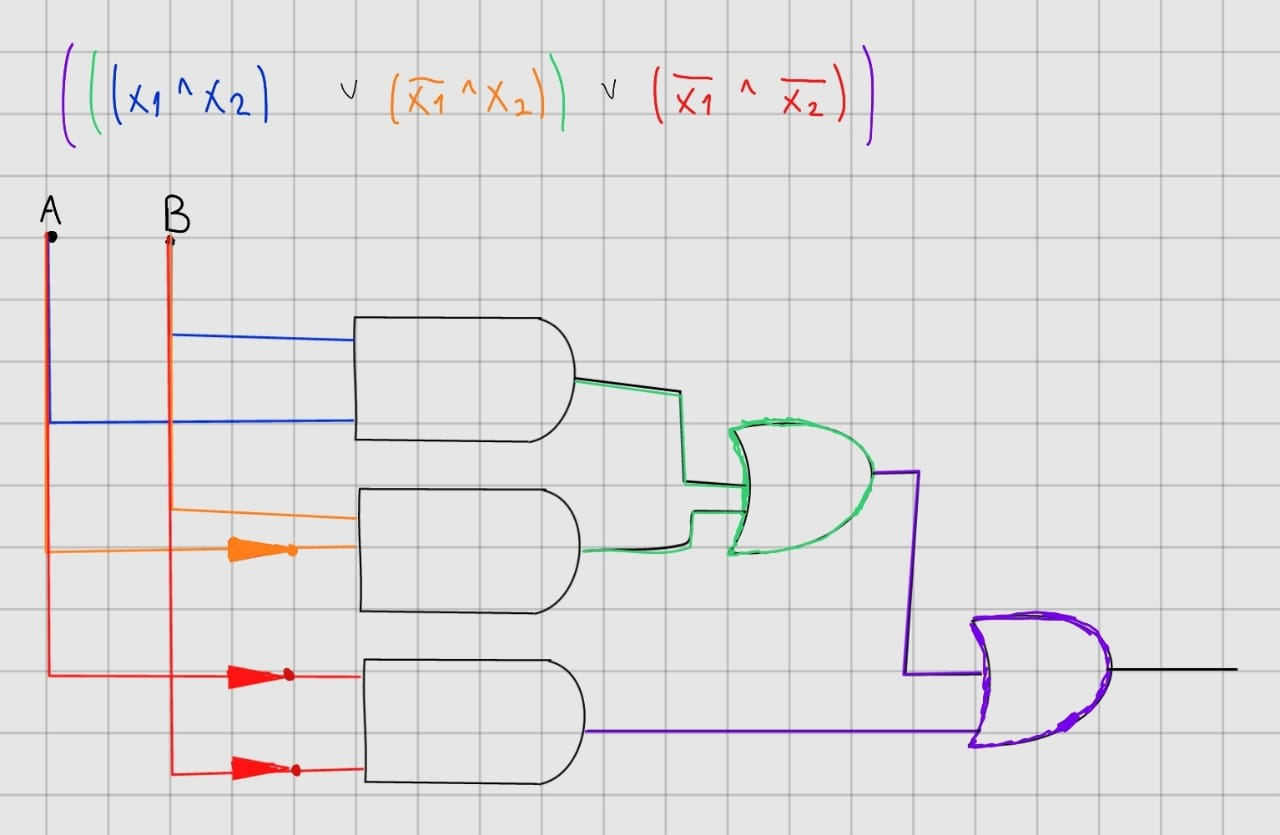
\includegraphics[width=\linewidth]{assets/circuito1.jpg}
    \label{fig:circuito1}
\end{minipage}\]

\subsection*{Carry en circuitos}
El carry debe colocarse en los circuitos en la suma porque en caso de no hacerlo, se nos pierden casos.
\[\begin{minipage}[b]{0.6\textwidth}
    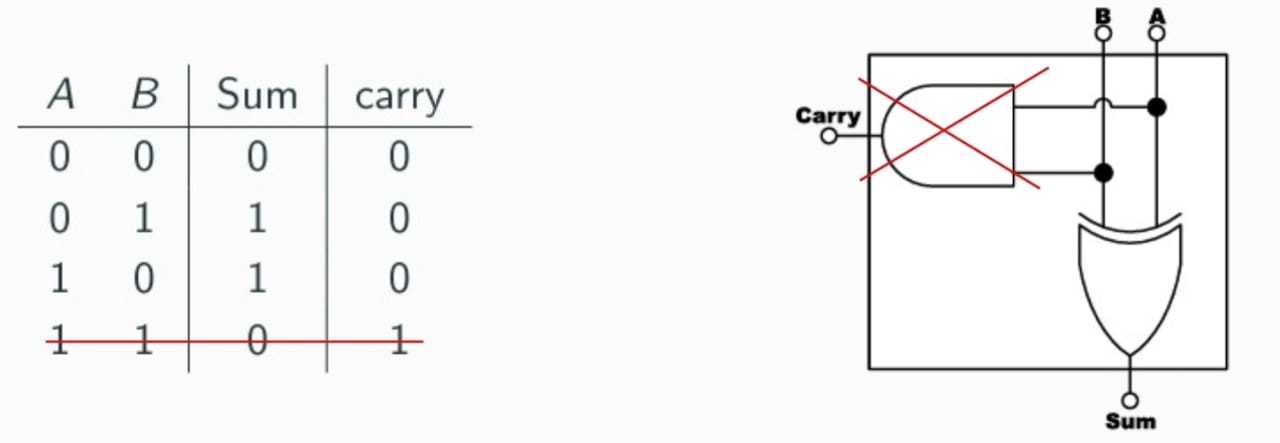
\includegraphics[width=\linewidth]{assets/sin_carry.jpg}
    \label{fig:sin_carry}
\end{minipage}\]

Si eliminamos el carry se nos pierde el caso 1 \( + \) 1, por lo tanto lo ideal sería que al hacer una suma nos quede así: 
\[\begin{minipage}[b]{0.6\textwidth}
    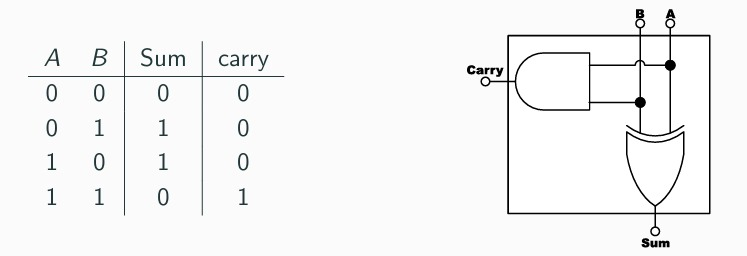
\includegraphics[width=\linewidth]{assets/suma_carry.jpg}
    \label{fig:suma_carry}
\end{minipage}\]

Nota: El carry es representado con un AND porque en la tabla de verdad solo da uno cuando A = 1 y B = 1. Luego, la función Sum es un XOR.

\subsection*{Sumadores}
Los sumadores nos sirven para poder realizar operaciones entre bits.
Es importante recalcar que llamamos half-adder a un sumador de 1 bit, donde solamente tiene una entrada A de 1 bit y una entrada B de 1 bit.
Un sumador de 1 bit requiere:
\begin{itemize}
    \item Dos entradas A y B de 1 bit
    \item Una compuerta XOR (para la suma): solo el resultado es 1 o 0
    \item Una compuerta AND (para el carry): si la suma del XOR es 1+1
\end{itemize} 
\[\begin{minipage}[b]{0.6\textwidth}
    \includegraphics[width=\linewidth]{assets/sumador_1_bit.png}
    \label{fig:sumador_1_bit}
\end{minipage}\]

Veamos un ejemplo con un sumador completo de 3 entradas: Si para dos entradas necesitabamos un sumador simple, para 3 entradas necesito 2. Porque es (A+B) y luego res+C
\[\begin{minipage}[b]{1\textwidth}
    \includegraphics[width=\linewidth]{assets/sumador_completo.png}
    \label{fig:sumador_completo}
\end{minipage}\]
Nótese que para considerar si es carry al final de toda la suma o no usamos un or porque nos basta con que uno haya arrojado carry.

\subsection*{Inversor}
\begin{itemize}
    \item Si me mandan INV=1 entonces tengo que invertir los bits.
    \item La manera de hacer esto es utilizando un XOR.
\end{itemize} 
\[\begin{minipage}[b]{0.6\textwidth}
    \includegraphics[width=\linewidth]{assets/inversor_4_bits.png}
    \label{fig:inversor_4_bits}
\end{minipage}\]


\subsection*{Multiplexor}
Está conformado por varias entradas de control y entradas de datos. Existe una única salida. Es una especie de switch/case en programación donde la condición del switch acá se llama entrada de control.
\begin{itemize}
    \item Entradas de control: se indican de la manera \(c_{n}\)
    \item Entradas de datos: se indican de la manera \(e_{n}\)
\end{itemize} 
Para poder calcular la cantidad de entradas de control \(c_{n}\) que necesito para una cantidad m de entradas de datos \(e_{m}\) hago el siguiente cálculo: m \(<\) \(2^{l}\) hasta que me pase por primera vez.
\begin{itemize}
    \item Entradas de datos: 30.
    \item Entradas de control: Necesito 5 entradas de control porque \(2^{5}\) es 32.
\end{itemize} 
Cada entrada de control tiene un índice que podemos decirle individuo, por ejemplo, si tengo \(2^{l}\) entradas tengo 32 posibles combinaciones.
\begin{itemize}
    \item Si tengo 00010 significa que la persona que está hablando la persona 2.
\end{itemize}

En los Multiplexores existen difurcaciones, que cuando llegamos a una de ellas se nos desvía el camino enviándonos a una compuerta. Si en algún momento se llega a un valor 0, entonces decimos que el camino ya finalizó.\\
\subsection*{Timing}
En un circuito combinatorio el tiempo que tarda la salida en estabilizarse depende de la cantidad de capas de compuertas (latencia). Para enfrentar el problema usamos secuenciales.
\section*{Latchs}
Utilizan realimentación, es decir, la salida de una compuerta como entrada de otra.
\subsection*{Latch RS}
Tiene dos entradas: S (Set) y R (Reset), y dos salidas, Q y \(\bar{Q}\) y consiste en dos puertas NOR conectadas por realimentación
El circuito es consistente permanece estable \(\iff\) S = R = 0.
Tabla de verdad del Latch
\begin{figure}[h]
    \begin{subfigure}{0.4\textwidth}
        \centering
        \includegraphics[width=0.7\linewidth]{assets/latch_circuito.png}
        \label{fig:latch_circuito}
        \end{subfigure}
    \begin{subfigure}{0.5\textwidth}
        \centering
    \includegraphics[width=0.5\linewidth]{assets/latch.png}
    \label{fig:latch}
    \end{subfigure}
    \end{figure}
    

Funciona como un memorizador
\begin{itemize}
    \item Cuando S está prendido entonces Q = 1.
    \item Cuando Q está prendido entonces \(\bar{Q}\) = 1.
    \item Si ninguno está prendido recuerda el estado anterior. 
    \item Si ambos están prendidos, Q = 0 y \(\bar{Q}\) = 0. Este caso no debería estar permitido porque la salida es inconsistente.
\end{itemize}

Para recordar el estado anterior usamos la notación de: \(Q \ast\) y \(\bar{Q} \ast \) \\

\textbf{Importante}: El valor de las salidas depende de la implementación del latch. Por lo tanto, un Latch con NAND no sería lo mismo que un Latch con NOR.

\subsection*{Latch JK}
Acepta todas las combinaciones posibles de las entradas.
\begin{itemize}
    \item Cuando J está prendido entonces Q = 1.
    \item Cuando K está prendido entonces \(\bar{Q}\) = 1.
    \item Si ninguno está prendido recuerda el estado anterior. 
    \item Si ambos están prendidos, niega el estado anterior (¡necesita que haya un estado anterior!)
\end{itemize}

\[\begin{minipage}[b]{0.8\textwidth}
    \includegraphics[width=\linewidth]{assets/latch_jk.png}
    \label{fig:latch_jk}
\end{minipage}\]

Cuando J y K son 1, la función realizada se denomina función de conmutación, la salida se invierte. 

El circuito oscila (estado inestable)

\subsection*{Latch D}
Es un almacén para un bit de datos. La salida del Latch D es siempre igual al valor más reciente aplicado a la entrada y por lo tanto la recuerda y la produce.

Tiene una entrada de datos y una de control.

Este circuito es estable en todos los estados pero los tiempos no se pueden predecir porque dependen de D y puede causar carreras si existe un lazo en el circuito externo

\begin{itemize}
    \item Cuando D está apagado y C está prendido, se memoriza C.
    \item Si ambos están prendidos, se memoriza D.
    \item En cualquier otro caso, devuelve el valor memorizado.
\end{itemize}

\[\begin{minipage}[b]{0.8\textwidth}
    \includegraphics[width=\linewidth]{assets/latch_d.png}
    \label{fig:latch_d}
\end{minipage}\]

\subsection*{Control de transición de estados: Clock}
\[\begin{minipage}[b]{0.8\textwidth}
    \includegraphics[width=\linewidth]{assets/clock_1.png}
    \label{fig:clock_1}
\end{minipage}\]
El clock que necesitamos utilizar es el 3ro. ¿Por qué? Porque nos interesa solamente memorizar o guardar los estados de los valores cuando el clock está en el pico. \\
No necesitamos estar constantemente escuchando cambios con el clock, sino que nos interesa solo en la subida.
\\
Para solucionar este problema, podemos utilizar un detector de pulso.
\begin{figure}[h]
    \begin{subfigure}{0.4\textwidth}
        \centering
        \includegraphics[width=0.8\linewidth]{assets/detector_pulso_1.png}
        \label{fig:detector_pulso_1}
        \end{subfigure}
    \begin{subfigure}{0.7\textwidth}
        \centering
    \includegraphics[width=0.6\linewidth]{assets/detector_pulso_2.png}
    \caption{Detector de pulso implementado usando una compuerta AND. }
    \label{fig:detector_pulso_2}
    \end{subfigure}
    \end{figure}
\\ Es importante notar, que el detector de pulso dará 1 (el pico) en algunos casos porque la compuerta NOT tiene un pequeño delay para poder negar la entrada. A continuación se muestra un ejemplo de esto.
\[\begin{minipage}[b]{0.6\textwidth}
    \includegraphics[width=\linewidth]{assets/detector_pulso_3.png}
    \label{fig:detector_pulso_3}
\end{minipage}\]
La línea punteada indica el tiempo que tardó la entrada en ser negada. En ese momento es donde se nos ejecutan los picos que nosotros necesitamos. \\
Si mandamos input = 1, el primer momento queda 1 AND 1 y el AND es verdadero, pero luego de un momento queda 1 AND 0 y ahora la señal vuelve a estar baja. Si fuese 1 AND 1 todo el tiempo tendríamos un clock constante y no necesitamos eso. \\
Todas las compuertas tienen delay porque al estar compuestas de silicio, tardan un poco en entrar en calor.\\

Veamos un ejemplo en Logisim usando registros y una ALU con el tema este de la secuencialidad a la hora de escribir en el pico del clock. \\
\[\begin{minipage}[b]{0.6\textwidth}
    \includegraphics[width=\linewidth]{assets/pico_1_escritura.png}
    \label{fig:pico_1_escritura}
\end{minipage}\]
\[\begin{minipage}[b]{0.6\textwidth}
    \includegraphics[width=\linewidth]{assets/pico_2_clock_apagado.png}
    \label{fig:pico_2_clock_apagado}
\end{minipage}\]
\[\begin{minipage}[b]{0.6\textwidth}
    \includegraphics[width=\linewidth]{assets/pico_3_escritura.png}
    \label{fig:pico_3_escritura}
\end{minipage}\]
\begin{itemize}
    \item Se activan las instrucciones de \texttt{Reg0\_Write}, \texttt{Reg0\_enableOut} (que permite exponer su valor a los demás) y se activa \texttt{ALU\_A\_WRITE} para que la ALU reciba el valor que expone \texttt{Reg0\_enableOut}.
    \item La primera operación que toma el clock en el flanco de subida es la escritura del número en \texttt{Registro\_00}.
    \item Al apagar el clock, todo sigue igual.
    \item Al encender el clock en el primer flanco de subida la ALU recibió el valor en \texttt{ALU\_A\_WRITE} del \texttt{Registro\_00} que expuso previamente en \texttt{Reg0\_enableOut}.
\end{itemize}
En circuitos secuenciales se niega el clock para que cada operación pueda tomarse el tiempo que necesita, caso contrario pasa basura.

\subsection*{Flip-Flop JK}
Está armado en base a Latch JK + Clock. \\
El Latch JK funcionará igual pero solo memorizará el valor sii el clock está en el flanco de subida.
\begin{itemize}
    \item Cuando J es 1 y el clock está prendido, se guarda el valor de J.
    \item Cuando K es 1 y el clock está prendido, se guarda el valor de K.
    \item Cuando el clock está apagado devuelve el valor de J/K guardado en el último pulso al clock. 
    \item Cuando el clock está apagado y J, K = 1 se niega el resultado guardado en el último pulso al clock.
    \item En cualquier otro caso, sucede el ítem anterior.
\end{itemize}
\subsection*{Flip-Flop D}
Está armado en base a Latch D + Clock. \\
El Latch D funcionará igual pero solo memorizará el valor sii el clock está en el flanco de subida.
\begin{itemize}
    \item Cuando el clock es 1, guarda el valor de D en ese instante.
    \item Cuando el clock está apagado, devuelve el valor de D guardado en el último pulso al clock. En criollo: Guarda el valor de D hasta que haya otro flanco de subida (ciclo) y guarde uno nuevo.
\end{itemize}

\[\begin{minipage}[b]{0.5\textwidth}
    \includegraphics[width=\linewidth]{assets/flip_flop_d.png}
    \label{fig:flip_flop_d}
\end{minipage}\]

Nota: \(1\uparrow\) indica que solo es se evalúa cuando está en el flanco de subida.
\subsection*{Registros}
Para poder escribir registros necesitamos una entrada de control Enable que nos permitirá decirle al Flip-Flop cuando nosotros queremos permitir que nos cambie el valor / escriba la memoria. \\
Este flag de Enable deberá ir en un AND con el Clock, entonces si Enable = 1 y el Clock está en 1, entonces se le permite al Flip Flop guardar el valor de la operación realizada.
\[\begin{minipage}[b]{0.4\textwidth}
    \includegraphics[width=\linewidth]{assets/flip_flop_d_enable.png}
    \label{fig:flip_flop_d_enable}
\end{minipage}\]

Recuerdo: El Flip Flop D solo almacena 1 bit. Si necesitaramos almacenar n bits (registro de n bits) necesitaríamos n Flip Flop D y UN solo Enable/Clock.

\subsection*{Componentes de Tres Estados}
Apagado, Encendido y Desconectado.
Al estado Desconectado le decimos que es de Alta Impedancia y se simboliza \textbf{Hi-Z}
\[\begin{minipage}[b]{0.6\textwidth}
    \includegraphics[width=\linewidth]{assets/tres_estados.png}
    \label{fig:tres_estados}
\end{minipage}\]
En la materia, una combinación basura de un componente de tres estados es que haya más de una entrada de control prendida con una misma entrada de dato. Esto es porque si bien en Logisim se acepta, no tendría sentido abrir dos conductos y mandar dos datos (iguales), la corriente siempre varía en algún momento y lo haría estallar. \\
\textbf{Nota}: Antes de prender cualquier entrada de control, hay que asegurarse que entrada de dato tenga el valor que deseamos cargar. 
\subsection*{Bus}
Nos va a servir para poder conectar varios componentes. Es una vía de n bits que van a estar conectando todos los componentes de nuestra arquitectura.
\[\begin{minipage}[b]{0.7\textwidth}
    \includegraphics[width=\linewidth]{assets/bus_componentes.png}
    \label{fig:bus_componentes}
\end{minipage}\]
Cada dispositivo sería cualquier operación, por ejemplo cada dispositivo podría ser un Flip-Flop D. \\ \\
Ej.: Si \(Dispositivo_{0}\) tendría el número 2 escrito en 4 bits (0010) y el \(Dispositivo_{1}\) tendría el número 4 escrito en 4 bits (0100) entonces el bus tendría el valor de 6. Esto es un problema, porque básicamente se está haciendo una especie de conjunción de todas las cosas y no siempre vamos a querer que se haga de esa forma. Aquí aparece un concepto importante llamado Recurso Compartido. \\ \\
Llamamos \textbf{recurso compartido} cuando tenemos más de un componente/dispositivo conectado en un mismo bus y necesitamos decidir quién usa cada componente. \\ \\
Para prender uno de los dispositivos y no los demás, bastaría con poner en 1 el dispositivo que quiero mientras que los demás en 0. 
\subsection*{Reset}
Coloca en 0 el componente. Comúnmente, el reset es asincrónico. \\
Para entender el concepto de asincrónico, véase \hyperref[subsec:reset_sincronico_asincronico]{reset asincrónico - sincrónico}
\subsection*{Write Enable y Enable Out}
Son dos instrucciones. No pueden pasar ambas a la vez. O escribimos, o leemos.
Cada vez que hacemos el cambio de estado de Enable Out o Write Enable, en algún momento deberán volver al estado anterior.

\subsection*{Esquema de interconexión de n registros}
Ahora nos queda realizar el esquema 
\[\begin{minipage}[b]{0.4\textwidth}
    \includegraphics[width=\linewidth]{assets/registro_fin.png}
    \label{fig:registro_fin}
\end{minipage}\]
Utilizo 3 Flip-Flop D con la posibilidad de escribir cuando el clock está activo y un botón de reset \\
Se añade un EnableOut para que se muestre el dato almacenado con lo armado en el paso 1 \\ \\
¿Como podríamos copiar el dato de R1 a R0? 
\begin{itemize}
    \item Utilizo Enable Out en R1 - EnableOut-1 \(\leftarrow\) 1
    \item Habilito WriteEnable en R0 - WriteEnable-0 \(\leftarrow\) 1
    \item Espero que el Clock esté funcionando en R0
    \item Deshabilito WriteEnable en R0 - WriteEnable-0 \(\leftarrow\) 0
    \item Deshabilito Enable Out en R1 - EnableOut-1 \(\leftarrow\) 0
\end{itemize}
De esta manera podemos pasar datos entre registros.

\section{Máquinas de estado}
Los circuitos secuenciales pueden ser pensados formalmente como una Máquina de Estados Finitos o FSM.
Una máquina de estados queda definida por: 
\begin{itemize}
    \item Una lista de estados.
    \item Un estado inicial.
    \item Una lista de funciones que disparan las transiciones en función de las entradas. 
\end{itemize}
\subsection*{Diagramas de estado}
Nos indican el comportamiento de los circuitos secuenciales en base al estado y como van avanzando
\[\begin{minipage}[b]{0.6\textwidth}
    \includegraphics[width=\linewidth]{assets/diagramas_estado.png}
    \label{fig:diagramas_estado}
\end{minipage}\]
Nota: \(x^{'}\) indica la variable negada.

\subsection*{FSM - Moore}
La salida depende solo del estado actual.
\begin{itemize}
    \item La salida siempre cambia un clock después que se dispara la condición de transición.
    \item No produce glitches a la salida.
    \item La cantidad de estados para reproducir cierto comportamiento puede ser más grande que con otro tipo de FSM.
\end{itemize}

\subsection*{FSM - Mealy}
La salida depende del estado actual y las entradas.
\begin{itemize}
    \item La salida pueda cambiar dentro del mismo clock en que se dispara la condición de transición.
    \item Produce glitches a la salida.
    \item La cantidad de estados para reproducir cierto comportamiento es más chica que en Moore.
\end{itemize}

\subsection*{Lógica de próximo estado}
\[\begin{minipage}[b]{0.6\textwidth}
    \includegraphics[width=\linewidth]{assets/registros_flip_flops.png}
    \label{fig:registros_flip_flops}
\end{minipage}\]
\[\begin{minipage}[b]{0.4\textwidth}
    \includegraphics[width=\linewidth]{assets/flip_flop_registros.png}
    \label{fig:flip_flop_registros}
\end{minipage}\]

¿Qué valores deberían tener \(D_{1} \ y \ D_{0}\) para obtener los valores deseados en el tiempo t+1, es decir, \(Q_{1}(t+1) \ y \ Q_{0}(t+1)\) \\
Usamos un flip-flop D, para que en vez de usar asignaciones dependa del estado anterior.
\[\begin{minipage}[b]{0.4\textwidth}
    \includegraphics[width=\linewidth]{assets/suma_productos_flip_flop_d.png}
    \label{fig:suma_productos_flip_flop_d}
\end{minipage}\]
\subsection*{Lógica de salida}
Consiste en hacer foco en como se deben vincular los estados porque muchas veces no nos es suficiente inferir comportamiento solo con la salida.
Veamos un claro ejemplo donde tenemos que hacer uso de la lógica de salida porque debemos conocer el estado para poder conocer el siguiente valor. 
00, 01, 11, y 10 son salidas.
\[\begin{minipage}[b]{0.4\textwidth}
    \includegraphics[width=\linewidth]{assets/logica_salida_ex.png}
    \label{fig:logica_salida_ex}
\end{minipage}\]
Para poder decidir esto, usamos etiquetas de estado.
\[\begin{minipage}[b]{0.6\textwidth}
    \includegraphics[width=\linewidth]{assets/logica_salida_etiquetas.png}
    \label{fig:logica_salida_etiquetas}
\end{minipage}\]
Nota: \(S_{n}\) n es el estado y el valor asignado es la codificacion. \\
TODO: Preguntar como hizo para calcular la suma de productos en base a los estados.
\[\begin{minipage}[b]{0.6\textwidth}
    \includegraphics[width=\linewidth]{assets/logica_salida_suma_productos.png}
    \label{fig:logica_salida_suma_productos}
\end{minipage}\]
\section{Arquitectura}
Observación: Nosotros vamos a manejarnos con 32 registros y data de 4 bytes.\\
¿Qué constituye una arquitectura?
\begin{itemize}
    \item El conjunto de instrucciones
    \item El conjunto de registros
    \item La forma de acceder a la memoria
\end{itemize}
Observación: Utilizaremos la arquitectura Risc V como programa de Assembler en la materia. \\
Observación 2: El lenguaje ensamblador depende de cada arquitectura. Cuando un lenguaje es compilado, traduce a la arquitectura de tu equipo.
\subsection*{Pasaje de lenguaje de alto nivel a bajo nivel}
Para esto se necesitan programas de compilado, ensamblado y enlazado.
\begin{itemize}
    \item El código de alto nivel es traducido por el compilador para pasar a código de bajo nivel.
    \item El código de bajo nivel es traducido por el ensamblador y se convierte en un código objeto (archivos \textbf{.o}).
    \item El código objeto es traducido por un enlazador y termina siendo binario ejecutable.
\end{itemize}
\subsection*{Aclaraciones sobre RISC V}
\begin{itemize}
    \item Las operaciones que contiene son las justas y necesarias, son pocas y la idea es que los problemas se resuelvan formando expresiones atómicas. 
    \item Los valores se extienden por el bit más significativo
    \item Las operaciones se llevan a cabo en el procesador.
    \item Todos los datos que se usan son de 32 bits.
    \item Los valores inmediatos toman como máximo, valores de 12 bits.
    \item Todas las operaciones que implican accesos a memoria, los valores inmediatos (se extienden a 12 bits) se indican en bytes. Ej: lw, sw. \\
    lw s7, 8(s3): el 8 RISC-V lo lee como 0000 0000 0100
    \item Todas las operaciones que implican operaciones aritméticas o lógicas, los valores inmediatos (se extienden a 12 bits) se indican en bits. Ej: srli
    \item Se acostumbra a decir 32 bits = 4 bytes = 1 palabra
\end{itemize}
\subsection*{Instrucciones atómicas y compuestas}
Es exactamente lo mismo que en lógica. Las operaciones se separan y deben indicarse claramente como se realizan.
Las instrucciones atómicas son aquellas que nos devuelven un valor irreducible, mientras que las instrucciones compuestas nos devuelven algo reducible. 
\subsection*{Operaciones en RISC V}
En RISC-V todas las instrucciones compuestas, se reducen a instrucciones atómicas antes de devolver el resultado. \\

\textbf{Importante}: Las instrucciones se guardan en la memoria RAM durante la ejecución del programa. Es decir, al ejecutar el programa carga todas las instrucciones de una en la RAM, luego, por cada línea que va pasando, agarra ese puntero a la RAM y hace el fetch \& decode \& execute.  \\

Reciben el nombre de mnemónico e indica el tipo de operación que queremos realizar. \\
Las operaciones reciben: \textbf{operandos de fuente} y un \textbf{operando destino}
\[a = b + c \equiv add \ a,\ b,\ c\]
El operando destino a sería el primer parámetro del mnemónico add, mientras que los operandos fuente serían b y c.
\subsection*{Comentarios en Risc V}
Usamos \# para comenzar una línea de comentarios.
\subsection*{Program Counter}
Recordatorio: Cada dirección se incrementa en múltiplos de 4 porque las instrucciones ocupan 4 bytes (1 palabra). \\
El procesador ejecuta el programa almacenando la posición de memoria de la instrucción que se está ejecutando en un registro de 32 bits conocido como el Program Counter. 
\subsection*{Registros en Risc V - Register File}
Viven en la CPU. \\ 
Cuenta con 32 registros que son implementados como un arreglo de memoria estática de 32 bits con varios puertos. \\
Los registros pueden nombrarse por su índice, desde x0 a x31 o según su uso habitual.
\begin{itemize}
    \item El registro zero (x0) almacena siempre el valor 0, y no puede ser escrito.
    \item Los registros s0 a s11 y los t0 a t6 se utilizan para almacenar variables: los registros pueden almacenar valores numéricos, direcciones de memoria a la RAM (punteros), punteros a funciones, etc.
    \item ra y de a0 a a7 tienen usos relacionados a llamadas de función.
\end{itemize}
\[\begin{minipage}[b]{0.4\textwidth}
    \includegraphics[width=\linewidth]{assets/PC.png}
    \label{fig:PC}
\end{minipage}\]
El registro PC es el Program Counter y lleva el registro de lo que se está ejecutando en un momento dado. Cuando un programa ya termina, el PC sigue apuntando a la posición de memoria de lo último que ejecutó. \\
Nota: los valores que toman las operaciones no pueden ser de 32 bits porque la operación en sí ya ocupa 5 bits. \\

\subsection*{Valores inmediatos}
Son valores constantes que se utilizan como operandos. Se encuentran disponibles en la misma instrucción y no hace falta recuperar su valor a partir de un registro o desde la memoria. \\
El valor puede escribirse en decimal, hexadecimal (prefijo 0x) o binario (prefijo 0b). \\
\textbf{Los valores inmediatos son de 12 bits y se extiende con el bit de signo a 32 bits antes de operar.}
\begin{itemize}
    \item \# s0 = a, s1 = b
    \item \(addi \ s0,\ s0,\ 4\) \# a = a + 4
    \item \(addi \ s1,\ s0, \ -12\) \# b= a - 12
\end{itemize}
En este caso, el 4 y el -12 son extendidos a 32 bits para poder operar. \\ 
\textbf{Ojo: cuando el número inmediato a representar no está en el rango de [-2048, 2047] ($2^{11} \ o \ 12 \ bits$) las operaciones deben realizar un addi y un lui (load upper immediate).} \\
Véase ejercicio en \hyperref[subsec:TPRVC]{\underline{anexo}}

\subsection*{Asignación}
Se hace zero + lo que queremos asignar. Consideremos que s0 = i
\begin{itemize}
    \item \(addi \ s0,\ zero,\ 4\) \# i = 4
\end{itemize}
\subsection*{Load Upper Immediate}
Mejor conocida como lui en RISC-V. Toma los primeros 20 bits. \\ 
Es útil para cuando queremos agregar un dato que excede el rango de 12 bits, para luego combinarlo con un addi y cargar los últimos 11 bits y poder representar el número deseado.
\subsection*{Control de valores inmediatos mayores a 12 bits (positivos)}
Como en RISC-V podemos cargar valores inmediatos de 12 bits, cuando ya agregamos un bit adicional tenemos que hacer dos operaciones: un lui y un addi. \\
Explicación genérica de como cargar un valor inmediato de 32 bits:
\begin{itemize}
    \item Agarra los primeros 20 bits en binario.
    \item Aplica un lui: carga los primeros 20 bits, pero antes extiende el número con 0's desde la izquierda. Luego, guarda el resultado del lui.
    \item Hace un addi utilizando el resultado del proceso anterior y los 12 bits menos significativos del número inicial (habiendo sido esta parte extendida a 32 bits).
\end{itemize}
\textbf{1}.  
Véase \hyperref[subsec:valores_inmediatos_32_bits]{anexo} para un ejemplo de esta aplicación de lui y addi con valores inmediatos mayores a 12 bits.
\subsection*{Control de valores inmediatos mayores a 12 bits (negativos)}
\[\begin{minipage}[b]{0.6\textwidth}
    \includegraphics[width=\linewidth]{assets/valores_inmediatos_neg.png}
    \label{fig:valores_neg}
\end{minipage}\]
Cuando dice que la parte baja se expresa como un número negativo ¿está tratando de decir que el valor inmediato de la suma es -1657?
\subsection*{Memoria}
Se estructura y se accede como si fuera un arreglo de elementos de 32 bits (4 bytes). El acceso a memoria es significativamente más lento que el acceso a registros pero nos permite guardar más data. \\
\subsection*{Lectura en Memoria} 
Instrucción lw (load word) \\ 
lw carga en destino, el valor que tiene un registro que tiene un puntero hacia la ram. \\ 
\[lw \ destino, \ desplazamiento(registroALeer)\]
Ejercicio TypeScript: 
\begin{lstlisting}
    const numbersArr: number[] = [1, 2, 3, 4, 5];
    const five: number = numbersArr[4];
\end{lstlisting}
Equivale en RISC-V a:
\begin{lstlisting}
    # s1: numbersArr -> cargado a traves de .data, s7: five
    lw s7, 20(s1)   
\end{lstlisting}
Donde el 20 sería el offset para movernos desde s1, es decir, 20 bytes (5ta palabra) 
Mapa mental: a \( \leftarrow \) b \\
\subsection*{Escritura en Memoria} 
Instrucción sw (store word) \\
sw guarda un contenido dado, en un registro que tiene un puntero hacia la ram. Es decir, pisa el valor.
\[sw \ registroAGuardar, \ desplazamiento(destino)\] 
Ejercicio TypeScript: 
\begin{lstlisting}
    const numbersArr: number[] = [1, 2, 3, 4, 5];
    numbersArr[2] = 8; 
\end{lstlisting}
Equivale en RISC-V a:
\begin{lstlisting}
    # s1: numbersArr -> cargado a traves de .data
    addi t1, 8, zero
    sw t1, 12(s1)   
\end{lstlisting}
Mapa mental: a \( \rightarrow \) b \\
\textbf{Importante: destino, en los casos de lw y sw debe ser un puntero a la RAM y debe haber sido inicializado.} \\
Véase \hyperref[subsec:punteros_ram_registros]{\underline{anexo}} para ver ejemplos más claros. 
\subsection*{Máscaras}
Una máscara es un valor binario que se utiliza para seleccionar, filtrar o modificar bits específicos dentro de un registro durante operaciones de manipulación de bits. Las máscaras se aplican en conjunto con operaciones lógicas. \\

Un ejemplo, utilizando la máscara \#0x00 $\rightarrow$ \#0x001010 AND \#0x00 = \#0x000000 \\

Si bien este es un ejemplo que deja mucho que desear, véase la sección de \hyperref[subsec:byte_particular_desplazamiento]{\underline{colores RGB para obtener un color en particular.}}
\subsection*{Instrucciones lógicas en RISC V}
Sean dos registros cualesquiera, las operaciones lógicas se hacen bit a bit. Su uso viene combinado con máscaras. \\
Ejemplo de XOR entre dos registros
\begin{table}[h!]
    \centering
    \begin{tabular}{|c | c | c | c| c|}
    \hline
    s1 & 0100 0110 & 1010 0001 & 1111 0001 & 1011 0111 \\ \hline
    s2 & 1111 1111 & 1111 1111 & 0000 0000 & 0000 0000 \\ \hline
    xor s5, s1, s2 & 1011 1001 & 0101 1110 & 1111 0001 & 1011 0111 \\
    \hline
    \end{tabular}
    \label{tab:xor}
\end{table} 
\\
Véase \hyperref[subsec:byte_particular_desplazamiento]{\underline{colores RGB para obtener un color en particular.}} donde se usa una máscara y la operación bit a bit and.
\subsection*{Instrucciones de desplazamiento}
Como son operaciones aritmético/lógicas, la unidad de desplazamiento es en bits.
\begin{itemize}
    \item sll (shift left logical): desplaza a la izquierda tantas unidades como se diga, como es logico se añaden 0's a la derecha.
    \item srl (shift right logical): desplaza a la derecha tantas unidades como se diga, como es lógico se añaden 0's a la izquierda.
    \item sra (shift right arithmetic): desplaza a la derecha tantas unidades como se diga, como es aritmético se añade el bit más significativo a la izquierda.
\end{itemize}
Nota: También existen las versiones de estas operaciones con el immediate (i) para usar una constante.
\begin{table}[h!]
    \centering
    \begin{tabular}{|c | c | c | c| c|}
    \hline
    s5 & 1111 1111 & 0001 1100 & 0001 0000 & 1110 0111 \\ \hline
    slli t0, s5, 7 & 1000 1110 & 0000 1000 & 0111 0011 & 1\textbf{000 0000} \\ \hline
    srli t0, s5, 17 & \textbf{0000 0000} & \textbf{0000 0000} & \textbf{0}111 1111 & 1000 1110\\ \hline
    srai t0, s5, 3 & \textbf{111}1 1111 & 1110 0011 & 1000 0010 & 0001 1100\\ \hline
    \end{tabular}
    \label{tab:desplazamiento_riscv}
\end{table} 
\subsection*{Byte en particular con desplazamiento de bits}
\label{subsec:byte_particular_desplazamiento}
Como hablamos de desplazamiento y byte en particular, sabemos que tendremos que hacer un desplazamiento de bits, y además de eso utilizar una máscara para tomar el bit que nos interesa. \\ 

Esto es súper útil en el ámbito de procesamiento de gráficos donde se debe cambiar la intensidad de un color, aplicar filtros o analizar la composición de colores en una imagen. \\

Un ejemplo para ponernos en contexto sería la forma de expresar los RGB colors con hexadecimal es decir, \#RRGGBB. \\
¿Cómo es que hacemos este proceso de $"$extraer un byte$"$? Consideremos que tenemos el color RGB \#0xFF0044 donde como anteriormente mencionamos, solo nos interesa \#FF0044 y en este caso en particular: 00. \\
Datos: 
var = \#FF0044 
\begin{itemize}
    \item Desplazamos la cantidad de bits necesarias para que el valor que queramos esté en los menos significativos.
    \begin{itemize}
        \item En este caso particular, tenemos que hacer un desplazamiento desde el 00 unos 8 bits (4 bits cada dígito en hexa) $ \rightarrow $ srli t0, var, 8
        \item El resultado es t0 = 0x00FF00
    \end{itemize}
    \item Aplicamos la máscara de 0xFF y guardamos el resultado
    \begin{itemize}
        \item En este caso particular, tenemos andi s2, t0, 0xFF.
        \item Luego, s2 tiene el valor de 00 (la intensidad del verde)
    \end{itemize}
\end{itemize} 
Véase \hyperref[subsec:desplazamiento_bits]{\underline{anexo}} para más ejemplos de desplazamiento con bits.
\subsection*{Control del flujo de ejecución}
Se va pisando el PC (Program Counter). 
\subsection*{Etiquetas en RISC V}
Nos permiten ponerle nombre a subproblemas; No ocupan memoria. \\

Véase ejercicio en \hyperref[subsec:ejercicios_con_saltos_condicionales_incondicionales]{\underline{anexo}}
\subsection*{Orden que toman las operaciones en memoria}
Las posiciones de memoria que ocupa cada instrucción se leen de arriba hacia abajo sin importar si hay un salto o no.
Ver ejercicio en \hyperref[subsec:TPRVC]{\underline{anexo}} 
\subsection*{Saltos condicionales}
Instrucciones que pisan el PC: 
\begin{itemize}
    \item beq(branch if equal): reemplaza el PC si los dos operandos son iguales.
    \item bne(branch if not equal): reemplaza el PC si los dos operando son distintos.
    \item blt(branch if less than): reemplaza el PC si el primer operando es menor que el segundo.
    \item bge(branch if greather than or equal): reemplaza el PC si el primer operando es mayor o igual al segundo.
\end{itemize}
\subsection*{Saltos incondicionales}
Instrucciones que pisan el PC: 
\begin{itemize}
    \item j (jump): actualiza el valor del PC con el operando provisto (inmediato de 20 bits extendidos en signo a 32).
    \item jal (jump and link): que almacena el valor actual del PC en el registro indicado en el primer operando y actualiza el valor del PC con el segundo operando (este se usa para llamar a una función, terminar y volver a ese link anterior).
\end{itemize}
Véase \hyperref[subsec:ejercicios_con_saltos_condicionales_incondicionales]{\underline{anexo}}
\subsection*{Funciones}
En RISC V la función llamadora puede utilizar los registros del a0 hasta a7 para enviar argumentos. La función llamada usa a0 para devolver el resultado. \\

La función llamada no debe interferir con el estado de la función llamadora, es decir, debe respetar los valores de los registros (s0 a s11) y el registro ra (dirección de retorno). \\

El stack de la función llamadora debe mantenerse invariante al ingresar a la función llamada.
\subsection*{Llamando funciones \& enviando parámetros}
Los inicializamos en la función llamadora, y luego en la función llamada simplemente accedemos a ellos. \\ 
Véase ejercicio en \hyperref[ejercicio:saltos_condicionales_argumentos]{\underline{anexo}}
\subsection*{Pila (stack)}
Es una parte de la memoria RAM que se utiliza para almacenar información temporaria. \\ 

RISC-V tiene su propio registro de stack pointer (sp), donde sp contiene una lista de elementos, donde cada elemento es un puntero a la RAM.  \\

\subsection*{Reglas de llamada}
\begin{itemize}
    \item Regla para la llamadora: Antes de llamar debe guardar los valores de los registros temporarios que necesite utilizar al retornar (t0-t6, a0-a7)
    \item Regla para la llamada: Si va a utilizar los registros permanentes (s0-s11, ra) debe guardarlos al comenzar y restaurarlos antes de retornar
\end{itemize}
\subsection*{Fetch \& Decode \& Execute}
Es el núcleo del ciclo de instrucciones de un CPU, asegurando que las instrucciones se recuperen de memoria, se interpreten y se ejecuten. \\
\begin{itemize}
    \item Fetch: El CPU recupera la siguiente instrucción (sabe cuál es gracias al Program Counter) a ejecutar desde la memoria. 
    \item Decode: El CPU interpreta la instrucción recuperada, detectando el opcode, operandos, operación a realizar, etc. Además, se generan las señales de control correspondientes para que la ejecución tenga la configuración necesaria.
    \item Execute: El CPU ejecuta la instrucción. Luego, se actualiza el PC.
\end{itemize}
\textbf{Nota}: Las instrucciones que se deben ejecutar a medida que el Program Counter avanza están almacenadas en la memoria RAM desde que el programa se ejecuta. \\
\textbf{Referencias}: 
\begin{itemize}
    \item ¿Cómo se interpretan las instrucciones de RISC-V?: TODO
    \item Proceso de Fetch, Decode y Execute \hyperref[subsec:datapath_example]{desde un punto de vista de microarquitectura}
\end{itemize}
\section*{Compilación, ensamblado y ejecución}
\subsection*{El mapa de memoria}
\[\begin{minipage}[b]{0.6\textwidth}
    \includegraphics[width=\linewidth]{assets/memory_map.png}
    \label{fig:memory_map}
\end{minipage}\]
\subsection*{Directivas de ensamblado}
\[\begin{minipage}[b]{0.6\textwidth}
    \includegraphics[width=\linewidth]{assets/directivas_ensamblado.png}
    \label{fig:directivas_ensamblado}
\end{minipage}\]
\subsection*{Inicialización de datos}
\[\begin{minipage}[b]{0.6\textwidth}
    \includegraphics[width=\linewidth]{assets/inicializacion_datos.png}
    \label{fig:inicializacion_datos}
\end{minipage}\]
Inicialización de datos en la sección .data que va a ubicar la información en lo que el mapa se muestra como Global Data.

Programa final con inicialización de los datos en RISC V
\[\begin{minipage}[b]{0.6\textwidth}
    \includegraphics[width=\linewidth]{assets/risc_v_ejercicio.png}
    \label{fig:risc_v_ejercicio}
\end{minipage}\]

\section*{Cosas a utilizar en Risc V (machete)}
\subsection*{Registros RISC-V}
\label{subsec:registros_riscv}
Viven en el procesador. \\
\[\begin{minipage}[b]{0.5\textwidth}
    \includegraphics[width=\linewidth]{assets/registros_riscv.png}
    \label{fig:registros_riscv}
\end{minipage}\] 
Nota: utilizar la escritura del registro de la izquierda es lo mismo que los de la derecha. Pero queda más claro usar los de la derecha. \\
Para más información, véase Página 21 Guia Práctica de Risc V
\subsection*{Mapa de opcodes RISC-V}
\label{subsec:ins_risc_v}
Página 18 de Guia Práctica de Risc V
\[\begin{minipage}[b]{0.6\textwidth}
    \includegraphics[width=\linewidth]{assets/ins_risc_v.png}
    \label{fig:ins_risc_v}
\end{minipage}\]
\subsection*{Formato de instrucciones en RISC-V}
La siguiente imagen puede ser abrumadora sin ningún tipo de contexto, pero no es nada complicado. \\
\[\begin{minipage}[b]{0.8\textwidth}
    \includegraphics[width=\linewidth]{assets/32_bit_instruction_rirsc_v.png}
    \label{fig:32_bit_instruction_rirsc_v}
\end{minipage}\]
Esta imagen es la que utiliza el procesador para hacer el proceso de \textbf{decode}, para poder entender qué es lo que realiza la instrucción almacenada en la RAM. Veamos como interpretar cada cosa. Iremos desde los campos que tienen en común. \\
\begin{itemize}
    \item opcode: Es el código de operación. Nos dice qué familia (I, R, S, B, U, etc) de operaciones tiene la operación. Puede encontrar las distintas familias en la \textbf{la última columna} de la imagen de \hyperref[subsec:ins_risc_v]{\underline{la sección anterior}}
    \begin{itemize}
        \item R: Utilizan dos registros como operandos fuentes (rs1, rs2) y uno como operando destino rd. El campo op junto con funct7 y funct3 determinan el tipo de instrucción codificada.
        \item I: Utilizan registros como operando fuente (rs1), un inmediato de 12 bits (imm) y uno como operando destino rd. El campo op junto con funct3 determinan el tipo de instrucción codificada.
        \item S (instrucciones de carga): Codifica un inmediato de 12 bits en la instrucción. El desplazamiento (offset) siempre se desplaza una posición a izquierda antes de sumarlo al PC ya que se encuentra siempre en posiciones pares. Ej: sw.
        \item B (instrucciones de saltos condicionales): Codifica un inmediato de 13 bits en la instrucción. El desplazamiento (offset) siempre se desplaza una posición a izquierda antes de sumarlo al PC ya que se encuentra siempre en posiciones pares. Ej: beq
        \item U (instrucciones de inmediato superior): Codifica un inmediato de 20 bits en la instrucción. El desplazamiento (offset) siempre se desplaza una posición a izquierda antes de sumarlo al PC ya que se encuentra siempre en posiciones pares.
        \item J (instrucciones de saltos incondicionales): Codifica un inmediato de 21 bits en la instrucción. El desplazamiento (offset) siempre se desplaza una posición a izquierda antes de sumarlo al PC ya que se encuentra siempre en posiciones pares.
    \end{itemize}
    \item rd (Read Destination): Es donde se debe almacenar el resultado, usualmente es un registro. Imaginemos que esos bits, en nuestra instrucción es 00101, pasamos el valor a decimal (5) y esto equivale al registro x5/t0. Puede más información en \hyperref[subsec:registros_riscv]{\underline{la sección de Registros}}
    \item func: Es el código de la función. Es importante que el código de la función también depende de la familia. Por lo tanto hay que ver familia + código de función. Puede encontrar las distintas funciones de familia en la \textbf{la 3ra columna} de la imagen de \hyperref[subsec:ins_risc_v]{\underline{la sección anterior}}. \\
    Por fuera de la tabla dice Familia + Operación. \\
    Ej: 101 rd 0110011 es: I srai
    \item rs1 (Source Register 1): Es el primer operando que se utiliza en una operación dada. Imaginemos que esos bits, en nuestra instrucción es 01001, pasemos el valor a decimal (9) y esto equivale al registro x9/s1 (luego que sabe el registro, debe buscar el valor).
    \item rs2: Misma idea que rs1, es el segundo operando fuente.
    \item immediate: Se utiliza para operaciones que tienen inmediatos. Como por ejemplo: addi, srli, srai. Imaginemos que esos bits, en nuestra instrucción es 0000 0000 0111, pasemos el valor a decimal (7). Luego, el valor inmediato que se quiere sumar es 7.
\end{itemize}
Nota: no hay más que dos operandos fuente porque las operaciones de RISC-V se hacen entre operaciones atómicas, es decir, en las cuales ya con una única operación podemos deducir el valor de verdad.
\section*{HDL}
Los lenguajes de descripción de hardware (HDL) son herramientas que nos permiten describir la estructura y comportamiento de nuestros diseños de forma sencilla, sintética y escalable a la hora de diseñar e implementar hardware industrial a gran escala.
Existen dos lenguajes dominantes actualmente: VHDL y System Verilog. 
\subsection*{Módulos}
Son bloques de hardware que tienen entradas y salidas además de un nombre. Se los puede describir de dos maneras:
\begin{itemize}
    \item Comportamental: Como se modifican las señales salida en base a la entrada y en qué estado queda el componente.
    \item Estructural: Como se vinculan sus entradas y salidas entre sí y describiendo la composición de diversos componentes (una cajita usa otra cajita).
    \item Ej: AND, OR, multiplexor o sumador son ejemplos de módulos.
\end{itemize}
\subsection*{¿Para qué sirve el código HDL?}
Es la fuente de dos procesos.
\begin{itemize}
    \item Simulación: Simula, a través de ondas como se comporta el programa dada una serie de entradas y verifica que la salida sea la esperada.
    \item Síntesis: Traduce el HDL a un conjunto de compuertas lógicas.
\end{itemize}
Véase \hyperref[subsec:SVL_S_S]{\underline{anexo}} para un ejemplo. \\ 
Nota: en System Verilog, cuando vemos algo de tipo logic[7:0] significa que es un vector de 8 bits donde el 7 es el MSB y el 0 el LSB.
\section*{Modelado comportamental}
\subsection*{Tipos de asignaciones}
\begin{itemize}
    \item =: asignación bloqueante (aka: síncrona). En microarquitectura es un circuito combinatorio. 
    \item $<$=: asignación no bloqueante (aka: asincrónica). En microarquitectura es un circuito secuencial que funciona con bloques always. 
\end{itemize}
Véase \hyperref[subsec:bloques_always]{\underline{bloques always}} para más información
\subsection*{Operadores de reducción}
Colapsan los bits de una señal de tamaño variable aplicando una operación lógica. \\
$assign \ y = \&a$ \\
Ejecuta una especie de and entre todos los valores que tiene a sin necesidad de hacer uno por uno (ej: a[7] \& a[6]...) \\
\subsection*{Asignación condicional}
Infiere un multiplexor de dos entradas, es idéntico al ternario de C 
\[assign \ y \ = \ s \ ? \ d1 \ : \ d0\] 
donde:
\begin{itemize}
    \item s: entrada de control
    \item y: salida 
    \item d0: op 00 
    \item d1: op 01
\end{itemize}
\subsection*{Asignación condicional compuesto}
Es un ternario anidado. Infiere un multiplexor de cuatro entradas, por lo tanto son dos ternarios hijos y uno padre.
$ assign \ y = s[1] \ ? \ (s[0] \ ? \ d3 : d2) : (s[0] \ ? \ d1 : d0)$
\subsection*{Variables internas}
Se realizan con logic dentro del módulo. \\
$logic \ p, \ g;$ $ \leftarrow  $ crea dos variables p y g. \\
Véase \hyperref[subsec:SVL_FullAdder]{\underline{anexo}} para un ejemplo con un full adder

\subsection*{Precedencia de operaciones}
También conocido como "prioridad" de operaciones.
\[\begin{minipage}[b]{0.6\textwidth}
    \includegraphics[width=\linewidth]{assets/precedencia_operaciones.png}
    \label{fig:precedencia_operaciones}
\end{minipage}\]
\subsection*{Valores numéricos}
\[bits' + base + valor\]
ej: 8b10 $ \rightarrow \ $ 8 bits, binario número 2 (0000 0010) \\ 
La base se indica con una sola letra: d (decimal), b (binario), o (octal), h (hexadecimal). \\
Nota: siempre se termina almacenando en binario. 
\subsection*{Alta Impedancia (Resistencia)}
En System Verilog se representa con el valor de z. \\
\begin{lstlisting}
    module buffer3(input logic[3:0] a, input logic enable, output tri[3:0] y);
        assign y = en ? a : 4'bz;
    endmodule
\end{lstlisting}
enable es una señal de control que dice si deja pasar la energía o no. Si está apagada entonces estaría en Hi-Z caso contrario, deja pasar el valor que tenga a. \\ 
Nota: Cuando enable es false, se le asigna 4'bz porque y es de 4 bits según la entrada al módulo ([3:0])
\subsection*{Valores desconocidos}
En SystemVerilog, cuando los valores de una señal no puede definirse y se considera como desconocida o como de valor x se puede valer a dos razones 
\begin{itemize}
    \item Valor no inicializado: La señal no se ha inicializado
    \item Contención: Cuando dos buffers de tres estados están conectados al mismo bus pero envían señales distintas.
\end{itemize}
Si sucede esto, indica un error en el diseño. 
\subsection*{Manipulación de bits}
\begin{itemize}
    \item \{\}: concatena bits. El número de afuera indica la cantidad de repeticiones. Ej: $ \{3\{d[0]\}\} \equiv d[0]d[0]d[0] $  
    \item \texttt{[]} accede a una lista específica de bits. Tienen que ser números descendentes. Es decir a $>$ b. Ej: c[a:b]
\end{itemize}
\begin{lstlisting}
    assign y = {c[2:1], {3{d[0]}}, c[0], 3'b101};
\end{lstlisting}
\section*{Modelado Estructural}
Para poder componer módulos, tenemos que hacer instancias de ellos. 
\[componente \ nombreInstancia(parametros)\] \\ 
Véase \hyperref[subsec:SVL_comp]{\underline{anexo}} para un ejemplo. \\
Nota: Utilizando el enfoque estructural, la implementación de un mismo comportamiento se puede conseguir como composición de distinto tipo de componentes. 
\subsection*{Circuitos Secuenciales}
Se describen con componentes de memoria y se emplean bloques always.
\subsection*{Bloques Always}
\label{subsec:bloques_always}
Utilizados para indicar frente a qué evento se debe actualizar el estado de cada componente. \\ 
Cada bloque always viene con una lista de eventos (sensitivity list) que les hace efecto.  \\
Nota: Si el bloque always tiene más de una asignación se las debe agrupar en un par begin end \\
\[bloque \ @(evento \ var)\] \\ 
Véase \hyperref[subsec:SVL_bloques_clk]{\underline{anexo}} para un ejemplo. 
\subsection*{Reset asincrónico - sincrónico}
\label{subsec:reset_sincronico_asincronico}
Reset asincrónico: Cobra efecto en cuanto cambia de valor la señal. \\ 
Reset sincrónico: Cobra efecto frente al evento del flanco ascendente del reloj.
\subsection*{Always Comb - Circuitos Combinatorios}
No entendí
\subsection*{Case - Circuitos Combinatorios}
Se usa igual que en los lenguajes de programación pero acá es simplemente case.
\begin{lstlisting}
    case(data):
     0: segments = algo;
     1: segments = algo; 
     ...
     default: segments = algo; 
    endcase
\end{lstlisting}
Nota: segments es una variable de salida de 7 bits.
\section*{Microarquitectura}
Es la parte más cercana a la ingeniería. Nos sirve para poder entender como se manejan los flujos de información entre assembler (algo más abstracto) a circuitos combinatorios y secuenciales (algo más visual). \\
La microarquitectura se va a encargar de actualizar los registros y el program counter. \\

\subsection*{Datapath}
Un camino de datos o datapath es un conjunto de componentes funcionales, que realizan operaciones de procesamiento de datos, registros y buses. Junto con la unidad de control forman una CPU. \\
\textbf{Pero, ¿quién es el encargado de controlar el orden de las operaciones en el DataPath?} la unidad de control. \\  
\subsection*{Componentes del DataPath y responsabilidades}
Glosario antes de empezar: 
\begin{itemize}
    \item A: Address
    \item RD: Read Destination
    \item WD: Write Destination
    \item WE: Write Enable 
\end{itemize}
El DataPath está formado por
\begin{itemize}
    \item Program Counter (CPU): Contiene la instrucción actual. PC Next: Si hay un salto condicional, entonces contiene la posición de memoria donde se encuentra el salto; en otro caso, se incrementan 4 bytes (una palabra).
    \item Instruction Memory (CPU): Recibe el address de la instrucción para poder hacerle el fetch (hacia la memoria RAM). Es decir, obtener la representación binaria de la operación.
    \item Control Unit (CPU): Es el director de orquesta. Es quién le dice a cada componente qué es lo que tiene que hacer, y qué es lo que sigue luego de haber terminado su responsabilidad.
    \item Register File (CPU): Contiene los 32 registros x0-x31. Posee dos puertos de lectura (RD1 y RD2) que vuelcan el valor de las entradas de escritura (A1 y A2) respectivamente. WD3 también es un puerto de entrada de escritura que escribe el dato en A3 durante el flanco ascendente del reoj si la señal de control WE3 se encuentra alta.
    \item Multiplexores (CPU)
    \item ALU (CPU)
    \item Buses de Datos (CPU)
    \item Data Memory (RAM)
\end{itemize}
Véase \hyperref[subsec:datapath_example]{\underline{anexo para un ejemplo de un datapath}} 
\subsection*{Colores en un Data Path}
\begin{itemize}
    \item Líneas gruesas: datos de 32 bits.
    \item Líneas delgadas: datos de 1 bit.
    \item Líneas intermedias: datos de otro tamaño.
    \item Líneas azules: señales de control 
\end{itemize}

\section*{Anexo - Ejercicios}
\subsection*{Hexadecimal en RISC-V}
Recuerde que en RISC-V operamos siempre con 32 bits. \\

¿Qué realiza la operación andi t0, 0xABCDE, 0xFFF? \\
Sé que cada dígito hexadecimal son 4 bits, por lo tanto, pasemos todo a binario para que tengamos un mejor panorama, pero lo que va a terminar sucediendo es que nos quedará 0x00CDE, osea 0xCDE. 
\begin{itemize}
    \item 0xABCDE $\equiv$ 0000  0000  0000 1010  1011  1100  1101  1110 
    \item 0xFFF $\equiv$ 0000  0000  0000  0000 0000  1111  1111  1111  
\end{itemize} 
Luego, \\
andi realiza la operación de AND y a ojo podemos ver, que en binario nos queda: t0 = 1100 1101 1110 que equivale a 0xCDE
\subsection*{Registros en lw y sw}
\label{subsec:punteros_ram_registros}
\begin{lstlisting}
    addi x1, x2, 3 -> 5
    sw x3, 0(x1) (se desplaza 0 bytes desde x1) -> se coloca el valor de x3 en x1
\end{lstlisting}
¿Es correcta esta implementación? Considere que x2 tiene es un registro que tiene el valor de 5. \\
No, la implementación no es correcta, porque se intenta escribir en x3, un supuesto puntero a la RAM x1, pero x1 es un valor. Esto sería un error grave. \\ 
\begin{lstlisting}
    lw x1, 8(x2) -> guarda en x1, la posicion de memoria de x2 corrida 2 palabras (desplaza 8 bytes).
    sw x3, 0(x1) -> almacena el valor de x3 en la posicion de memoria de x1 (desplaza 0 bytes)
\end{lstlisting}
¿Es correcta esta implementación? Considere que x2 tiene es un registro que tiene un puntero a la RAM, tal que su valor decodificado es 5. \\
Sí, la implementación es correcta. Porque toma el registro x2 que tiene un puntero a la memoria, lo corre dos palabras y lo almacena en x1. Luego, x1 (que tiene una nueva dirección de memoria a la RAM (puntero)) lo guarda en x3. \\ 
\begin{lstlisting}
    lw x1, 256(x2) -> guarda en x1, la posicion de memoria de x2 corrida 2 palabras (desplaza 8 bytes).
    sw x3, 0(x1) -> almacena el valor de x3 en la posicion de memoria de x1 (desplaza 0 bytes)
\end{lstlisting}
¿Es correcta esta implementación?
\subsection*{Desplazamiento de Bits para obtener un Byte particular}
\label{subsec:desplazamiento_bits}
Almacene, en un registro cualesquiera el segundo byte del siguiente hexadecimal: \#0x89ABCDEF sabiendo que el valor está en la memoria RAM; indique qué datos son relevantes, y qué mascara utilizará. \\
Datos: \#89ABCDEF \\
Sé que cada dígito hexadecimal son 4 bits, por lo tanto, si tengo que sacar el segundo byte: 4 + 4 = 8 bits (1 byte) por lo tanto tengo que sacar CD pues (4 + 4 + 4 + 4 = 16 $ \equiv $ 2 bytes) \\
Sé que como CD debo llevarlo a los más significativos, aplico un srli 8 bits a la derecha.
Sé tambien que si el valor es una posición de memoria en la RAM, voy a tener que usar li pues necesito cargarlo desde la memoria principal (RAM). \\
Tengo que utilizar la máscara 0xFF (Rdo que al ser 32 bits, los últimos 8 son 1) con (\#11111111) con un and pues necesito aislar los bytes que me interesan. \\
¿Por qué una máscara? porque una máscara se utiliza para seleccionar ciertos bits, descartando los que no necesitamos. Las máscaras las aplicamos haciendo operaciones lógicas bit a bit como AND, OR, XOR, NOT, entre otras.
Código en RISC-V
\begin{lstlisting}
    li t0, 0x89ABCDEF
    srli t1, t0, 8 (desplazamiento logico de 8 bits a la derecha) <- 0x0089ABCD
    andi t1, t1, 0xFF <- 0x0000CD <- 0xCD
\end{lstlisting}
\subsection*{Control de valores inmediatos mayores a 12 bits $2^{11} (12 \ bits)$}
\label{subsec:valores_inmediatos_32_bits}
\begin{itemize}
    \item 0xABCDE123 ¿excede los 12 bits para ser un inmediato? Pasemos a binario
    \begin{itemize}
        \item 0001 0010 0011 0100 0101 0110 0111 1000
        \item Sí, excede los 12 bits; Por lo tanto tenemos que usar un lui y un addi para cargarlo.
    \end{itemize}
    \item De ese binario gigante, hago un lui de los 20 más significativos \& addi de los 12 menos significativos.
    \item Entonces, si seguimos en binario nos queda algo así:
    \begin{itemize}
        \item lui s2, 0001 \ 0010 \ 0011 \ 0100 \ 0101 como acá tengo 20 bits pero estoy en 32 bits, extiendo con 0's. \\ Rta: 0001 \ 0010 \ 0011 \ 0100 \ 0101 \ 0000 \ 0000 \ 0000
        \item addi s2, s2, 0110 0111 1000. \\ Rta: 0001 0010 0011 0100 0101 0110 0111 1000
    \end{itemize} 
    \item En Hexa:
    \begin{itemize}
        \item lui s2, 0xABCDE (nótese que cada letra son 4 bits, 4 * 5 = 20 bits). \\ Rta: 0xABCDE000 (nótese que se agregaron tres ceros, porque son lo que falta para llegar a 32 bits).
        \item Luego que nuestro s2 ya tiene los ceros para pisar, cargo la parte baja con addi: addi s2, s2, 0x123. \\ Rta: 0xABCDE123 
    \end{itemize}
\end{itemize}
\label{subsec:}
\subsection*{Ejercicios con Saltos Condicionales / Incondicionales}
\label{subsec:ejercicios_con_saltos_condicionales_incondicionales}
Ejercicio llamado a procedimiento sin retorno,
TypeScript: Salto sin retorno, y modificación de variable global. 
\begin{lstlisting}
    let destinatarios = 2;

    while(destinatarios>0){
       destinatarios -= 1;
    }
\end{lstlisting}
Equivale en RISC-V a:
\begin{lstlisting}
    #s2 = destinatarios
    lw a0, s2 
    j loop
    loop: 
        addi a0, a0, -1
        beq a0, zero, fin 
        j loop
    fin:  
\end{lstlisting}
\label{ejercicio:saltos_condicionales_argumentos}
Ejercicio con recursión, 
TypeScript: Salto con retorno, y modificación de variable global. 
\begin{lstlisting}
    let destinatarios = 2;

    const hacerCero = (destinatarios: number): number => {
        if(destinatarios == 0) return 0; 
        return hacerCero(destinatarios-1);
    }

    const respuesta: number = hacerCero(destinatarios);
\end{lstlisting}
Equivale en RISC-V a:
\begin{lstlisting}
    #s2 = destinatarios
    lw a0, s2                               #0x0000 0000
    jal ra, hacerCero                       #0x0000 0004
    sw v0, x3                               #0x0000 0008
    ecall                                   #0x0000 000C
    hacerCero: 
        addi sp, sp, -4                     #0x0000 0010
        sw ra, 0(sp)                        #0x0000 0014 
        beq a0, zero, finHacerCero          #0x0000 0018
        addi a0, a0, -1                     #0x0000 001C
        jr hacerCero                        #0x0000 0020
    finHacerCero: 
        li v0, 0                            #0x0000 0024
        lw ra, 0(sp)                        #0x0000 0028
        sw sp, 4(sp)                        #0x0000 002C
        jr ra                               #0x0000 0030
\end{lstlisting}
\textbf{Nótese}: que al usar recursión, reservamos siempre 4 bytes para guardar el ra por si llegamos a saltar a otra función en el beq. \\
\textbf{Nótese}: a0 se puede utilizar en hacerCero pues, a0 previo a una llamada a una función sería un argumento.
\subsection*{Hexa - Binario - Risc V}
\textbf{Decodifique a instrucciones de RISC-V} \\
1. $0x00700293$ \\ 

\textbf{Pasamos cada numero hexadecimal a binario, cada hexa son 4 bits de binario} \\ 
$0000 \ 0000 \ 0111 \ 0000 \ 0000 \ 0010 \ 1001 \ 0011$ \\

\textbf{Ahora sabemos que el opcode son los últimos 7 bits, reagrupamos} \\ 
$0000 \ 0000 \ 0111 \ 0000 \ 0000 \ 0010 \ 1 \ 0010011$ \\

\textbf{Vemos que familia de operación corresponde a 0010011 en la tabla de la Figura 2.3. La familia es $ \implies $ I} \\
\textbf{Ahora vemos que lo que le sigue es el rd, por lo tanto reagrupo} \\
$0000 \ 0000 \ 0111 \ 0000 \ 0000 \ 00101 \ 0010011$ \\

\textbf{Lo que sigue ahora es la func, que son 3 bits, por lo tanto reagrupo} \\
$0000 \ 0000 \ 0111 \ 0000 \ 0 \ 000 \ 00101 \ 0010011$ \\

\textbf{Lo que sigue ahora es el rs1 que toma 5 bits, por lo tanto reagrupo} \\ 
$0000 \ 0000 \ 0111 \ 00000 \ 000 \ 00101 \ 0010011$ \\ 

\textbf{Lo que sigue ahora es el immediate (20 a 31) porque estamos en la familia del I, por lo tanto reagrupo} \\ 
$0000 0000 0111 \ 00000 \ 000 \ 00101 \ 0010011$ \\

\textbf{Por último, traducimos a operaciones de RISC-V} \\ 
0010011 000: ADDI  \\ 
00101 rd: pasado a decimal es 5, por lo tanto en la tabla de registros x5 es t0. \\
00000 rs1: pasado a decimal es 0, por lo tanto en la tabla de registros x0 es zero. \\
0x007: es donde se guarda en memoria, eso en decimal es 7 por lo tanto en la tabla de registros x7 es t2. \\ 

\textbf{Luego, juntamos todos los operandos en RISC-V} \\ 
ADDI t0, zero, t2

\subsection*{Traducción de programa de Risc V a castellano y observando las posiciones de memoria de instrucciones}
\label{subsec:TPRVC}
\begin{lstlisting}
    li a0, 4228 <- 0x0000 a 0x0008 (0 a 8) sin incluir
    li a1, 2114 <- 0x0008 a 0x0010 (8 a 16) sin incluir
    jal ra, resta <- 0x0010
    fin: 
        beq zero, zero, fin <- 0x0014
    resta: 
    prologo:
        addi sp, sp, -4 <- 0x0018
        sw ra, 0(sp) <- 0x001c
        sub a0, a0, a1 <- 0x0020
        beq a0, zero, epilogo <- 0x0024
    sigo: 
        jal ra, resta <- 0x0028
    epilogo:
        lw ra, 0(sp) <- 0x002c
        addi sp, sp, 4 <- 0x0030
        ret <- 0x0034
\end{lstlisting}
\textbf{Nota}: Recordar que las etiquetas no son funciones, son simplemente instrucciones que se leen. Es decir, por ejemplo, cuando va por prologo y llega a beq si es falso ejecuta sigo, pero no es necesario llamarla sino que lo de jal ra, resta es parte del prologo solo que se le dio un subnombre. Todo se lee de arriba hacia abajo, por lo tanto a epilogo tambien estaría dentro de prologo por así decirlo pero nunca llega porque el beq si es falso hace llamada recursiva. Solo llega a epilogo y cambia el PC si el beq es true. \\ 
Nota: fin ¿no termina nunca cierto? es re contra recursivo
¿Qué hace este código? línea por línea
\begin{itemize}
    \item li a0, 4228: carga el valor de 4228 en el registro a0. Internamente son dos operaciones, lui y addi por lo tanto ocupan desde 0x0000 a 0x0008 (sin incluir).
    \item li a1, 2114: carga el valor de 2114 en el registro a1. Internamente son dos operaciones, lui y addi por lo tanto ocupan desde 0x0000 a 0x0010 (sin incluir)
    \item jal ra, resta: salta a la etiqueta de resta y guarda la dirección de retorno en ra (para que el return de resta vuelva acá)
    \item addi sp, sp, -4: reserva 4 bytes en el stack pointer bajándolo. Esto es un caso específico, podría bajar 8 bytes si se quisiera pero como solo quiere escribir un solo valor, basta con 4 bytes. Importante que luego de hacer todo el stack debe volver a su posición original.
    \item sw: guarda ra en la primera posición del stack pointer. esto es porque luego cuando salta a epilogo tiene que saber bien a donde volver.
    \item sub: guarda en a0 la resta entre a0 y a1.
    \item beq: verifica si a0 es igual a zero, si es igual a cero salta a epilogo, caso contrario hace una llamada recursiva nuevamente a resta.
    \item sigo: si beq es falso llega acá, hace la llamada recursivamente como en la inicial mandando un nuevo estado.
    \item lw: se guarda en ra el valor que estaba en 0(sp) cuando lo guardamos antes.
    \item addi: vuelve a subir el stack a su posicion inicial porque ya no necesitamos hacer nada (nótese que es importante que subimos dejando todo como estaba pero nuestro ra que habiamos guardado antes en la primera pos lo recuperamos con el lw)
    \item ret: vuelve a jal ra, resta y ejecuta fin.
    \item el programa termina si zero es igual a zero pero luego ejecuta fin recursivamente. (no termina nunca)
\end{itemize}
Preguntas: 
\begin{itemize}
    \item a) Indicar en qué posiciones de memoria se encuentra cada etiqueta
    \begin{itemize}
        \item fin: 0x0014
        \item resta: 0x0010
        \item sigo: 0x0028
        \item epilogo: 0x002c
    \end{itemize}
    \item b) Hecho arriba 
    \item c) TODO
    \item d) TODO 
    \item e) ¿Cual es el valor final de a1? El valor final de a1 sería 0, pues dejaría de hacer el paso recursivo y llegaría a 0.
    \item f) ¿Cuál es el valor final del PC? El último valor del PC es la última instrucción que ejecutó, sería 0x0014 (fin).
    \item g) Listar la secuencia descripta por el PC. 0x0000 0x0004 0x0008 0x0010 0x0018 0x001c 0x0020 0x0024 0x0028 (vuelve a entrar a prologo) 0x0018 0x001c 0x0020 0x0024 (evalua guarda, true va directo a epilogo) 0x002c 0x0030 0x0034 (el return nos manda de vuelta al jal) 0x0010 0x0014 (fin)
    \item h) Indique qué valores toman los registros ra y sp: al inicio, durante y al finalzar la ejecución
    \begin{itemize}
        \item ra: 0x0010 antes de saltar a resta, dentro del prologo, ra se guarda en la primera posicion del sp ocupando los primeros 4 bytes, finalmente en epilogo, a ra se le coloca la posición del elemento 0 del stack pointer. De igual manera, ra siempre tiene el mismo valor, nunca cambia.
        \item sp: Se desconoce que tiene inicialmente pero tiene cosas de memoria dinámica, variables globales, otras instrucciones, etc. Pero viendo solo el programa, el sp se mueve hacia abajo 4 bytes. Luego, en el espacio que reservamos se guarda el valor de ra. Por ultimo, los primeros 4 bytes del stack pointer se almacenan en ra y se liberan los 4 bytes que habíamos reservado.
    \end{itemize}
    \item i) Reemplazar la segunda instrucción li a1, 1023 de modo que a1 sea a0 dividido 2 con una única instrucción (acá hay algo raro porque la segunda instrucción no es a1, 1023 es a1 2114)
\end{itemize}
Pasemos esto a TypeScript: A modo ilustrativo, si la función recursiva termina retornará true, caso contrario se quedaría colgada. En estos casos siempre termina xq los números dan.
\begin{lstlisting}
    const a0:number = 4228;
    const a1:number = 2114;

    const resta = (a0: number, a1: number): number | boolean => {
        if(a0 == 0){
            return true; //epilogo
        }
        else{
            return resta(a0-a1, a1);  //sigo
        }
    }

    const res = resta(a0, a1);
    console.log(res); //true
\end{lstlisting}
\subsection*{System Verilog - Síntesis - Simulación}
\label{subsec:SVL_S_S}
\begin{lstlisting}
    module compuertas(
        input logic [3:0] a, b,
        output logic [3:0] y1, y2, y3, y4, y5
        );

        assign y1 = a & b; //and
        assign y2 = a | b; //or
        assign y3 = a ^ b; //xor
        assign y4 = ~(a & b) (alt gr y simbolo de ~ para escribirlo) //nand
        assign y5 = ~(a | b); //nor
    endmodule 
\end{lstlisting}
Nota: [3:0] son 4 bits donde 3 es el bit más significativo (MSB) y 0 el menos significativo (LSB)
Circuito sintetizado:
\[\begin{minipage}[b]{0.6\textwidth}
    \includegraphics[width=\linewidth]{assets/circuito_sintetizado.png}
    \label{fig:circuito_sintetizado}
\end{minipage}\] 
\subsection*{System Verilog - Síntesis (Full Adder)}
\label{subsec:SVL_FullAdder}
\begin{lstlisting}
    module fulladder(input logic a, b, cin, output logic s, cout);
        logic p, g; 
        assign p = a ^ b;
        assign g = a & b;
        assign s = p ^ cin;
        assign cout = p | (p & cin);
    endmodule
\end{lstlisting}
\[\begin{minipage}[b]{0.6\textwidth}
\includegraphics[width=\linewidth]{assets/sintesis_full_adder.png}
\label{fig:sintesis_full_adder}
\end{minipage}\] 
\subsection*{Composición de multiplexores - Comportamiento Estructural}
\label{subsec:SVL_comp}
\begin{lstlisting}
    module mux4(input logic [3:0] d0, d1, d2, d3, input logic[1, 0] s, output logic [3:0] y);
    logic [3:0] low, high;
    mux2 lowmux(d0, d1, s[0], low);
    mux2 highmux(d2, d3, s[0], high);
    mux2 finalmux(low, high, s[1], y);
\end{lstlisting}
Nótese que lowmux, highmux y finalmux son instancias de mux2.
\subsection*{System Verilog - Asignación no bloqueante}
\label{subsec:SVL_bloques_clk}
\begin{lstlisting}
    module flop(input logic clk, input logic [3:0] d, output logic[3:0] q);
        always_ff @(posedge clk)
        q < = d;
    endmodule
\end{lstlisting}
La asignación no bloqueante de d en q se hace cuando ocurre el evento posedge clk, lo que significa que se actualiza el estado en el flanco ascendente de la señal del clock.
\subsection*{DataPath, ejemplo con instrucción Risc V}
\label{subsec:datapath_example}
¿Cómo se conecta Risc V con el DataPath? 
\begin{lstlisting}
    ADD x1, x2, x3 <- suma x2 y x3 y lo guarda en x1
\end{lstlisting}
\textbf{El paso a paso}: 
\begin{itemize}
    \item El PC se coloca sobre la instrucción
    \item Fetch: Gracias a la dirección proporcionada por el PC, busca la operación en la memoria RAM.
    \item Decode: Recibe la operación de la memoria RAM, y la interpreta en base al instruction format. La instruction memory, quien es encargado de este proceso, le pasa el control al siguiente. 
    \item Execute: Una vez que se decidió que debe realizarse, ejecuta las operaciones correspondientes en el orden. Quien dicta el orden y prioridades es la control unit, y el CPU quien las ejecuta.
    \begin{itemize}
        \item Toma las posiciones de memoria de x2 y x3; las solicita en el registro para obtener el valor; se envían los valores de x2 y x3 en binario, y una flag que le indica qué operación realizar a la ALU (ordenado por la unidad de control)
        \item El clock cambia de estado. 
        \item La ALU devuelve el resultado directamente al Register File (ordenado por la unidad de control), enviando el resultado a WD3 (Write Destination).
        \item WE3 se enciende (por aviso de la unidad de control); el clock cambia de estado, escribiendo en WD3 el resultado de la ALU.
    \end{itemize}
    \item El clock cambia de estado. 
    \item Al no haber un salto condicional, PCNext está vacío e incrementa el PC actual 4 bytes (1 palabra) (ordenado por la unidad de control) para leer la instrucción. En este caso, termina el programa. 
\end{itemize}

\end{document}
